% Results archived at d13c1a0c3131ba81adbeb911a50aa3f92d5aafe9.
% Numeric tables are generated from the unmodified JSON files in
% ../evidence/digits/ by ../scripts/build_digits_tables.py.
\clearpage
\section{Component and Gradient Diagnostics on Digits}
\label{app:digits_diagnostics}

We use the five calibrated FusedSpaceFed runs (seeds 42--46) reported in
Sections~\ref{sec:feature_heterogeneity_digits} and \ref{sec:capacity_compute}.
The data partition, architecture, and validation-selected hyperparameters
are those in Appendices~\ref{app:capacity_compute_comparison} and
\ref{app:feature_heterogeneity_digits}. The full-model reference is therefore
the same $85.86\pm0.85\%$ uniform-domain accuracy reported in the main text.

\subsection{Decoder Behavior and Reconstruction Warm-Up}
\label{app:digits_decoder}

What role does reconstruction warm-up play before task-driven optimization?
We replay one local participation from copies of the initial and final
(round 300) checkpoints of the five full-model runs, using a fixed training
probe of 160 examples per domain, arranged in five batches of 32.
Each replay performs one encoder-only warm-up epoch followed by one
end-to-end classification epoch. Optimizers are reset at the start of
participation, as in the Digits training protocol, with continuous Adam
state between the two phases. Metrics are evaluated with frozen BatchNorm
statistics. The intermediate states are local diagnostic replays from the
saved checkpoints.

Warm-up reduces reconstruction MSE averaged across seeds in every domain
at both checkpoint stages (Table~\ref{tab:digits_reconstruction}).
At the final checkpoints, MSE averaged across domains and seeds decreases
from 0.4512 to 0.4477 after warm-up, then increases to 0.5028 after
classification. These observations illustrate the distinct roles of the
two phases: warm-up improves reconstruction, whereas subsequent
classification shapes the decoder output through the prediction objective
alone.

\begin{table*}[t]
\coauthorcolor
\centering
\small
\setlength{\tabcolsep}{8pt}
\caption{Reconstruction MSE on the fixed Digits training probes, averaged over five seeds. Each checkpoint is copied before a local replay. Before, Warm-up, and Classification denote successive replay states; the two column groups start from initialization and round 300.}
\label{tab:digits_reconstruction}
\begin{tabular}{lrrrrrr}
\toprule
& \multicolumn{3}{c}{Initial checkpoints} & \multicolumn{3}{c}{Final checkpoints} \\
\cmidrule(lr){2-4}\cmidrule(lr){5-7}
Domain & Before & Warm-up & Classification & Before & Warm-up & Classification \\
\midrule
MNIST & 0.9428 & 0.9213 & 0.9239 & 0.9023 & 0.8962 & 1.1163 \\
SVHN & 0.1965 & 0.1921 & 0.1924 & 0.1877 & 0.1853 & 0.1955 \\
USPS & 0.5946 & 0.5804 & 0.5813 & 0.5649 & 0.5611 & 0.5715 \\
SynthDigits & 0.3730 & 0.3656 & 0.3670 & 0.3517 & 0.3482 & 0.3668 \\
MNIST-M & 0.2845 & 0.2795 & 0.2772 & 0.2496 & 0.2475 & 0.2639 \\
\bottomrule
\end{tabular}
\end{table*}


The decoder ends with a linear convolution, allowing output values beyond
the normalized input range $[-1,1]$. Figure~\ref{fig:digits_decoder_probe}
illustrates the image-space signals before and after each phase.
All measured outputs, losses, and model states remain finite in these
replays. During warm-up, only the encoder changes; classification updates
the encoder, decoder, and classifier.

\begin{figure*}[t]
\coauthorcolor
\centering
\setlength{\tabcolsep}{5pt}
\begin{tabular}{rccccc}
 & MNIST & SVHN & USPS & SynthDigits & MNIST-M \\
\raisebox{.20in}{\scriptsize\shortstack[r]{Input}} & 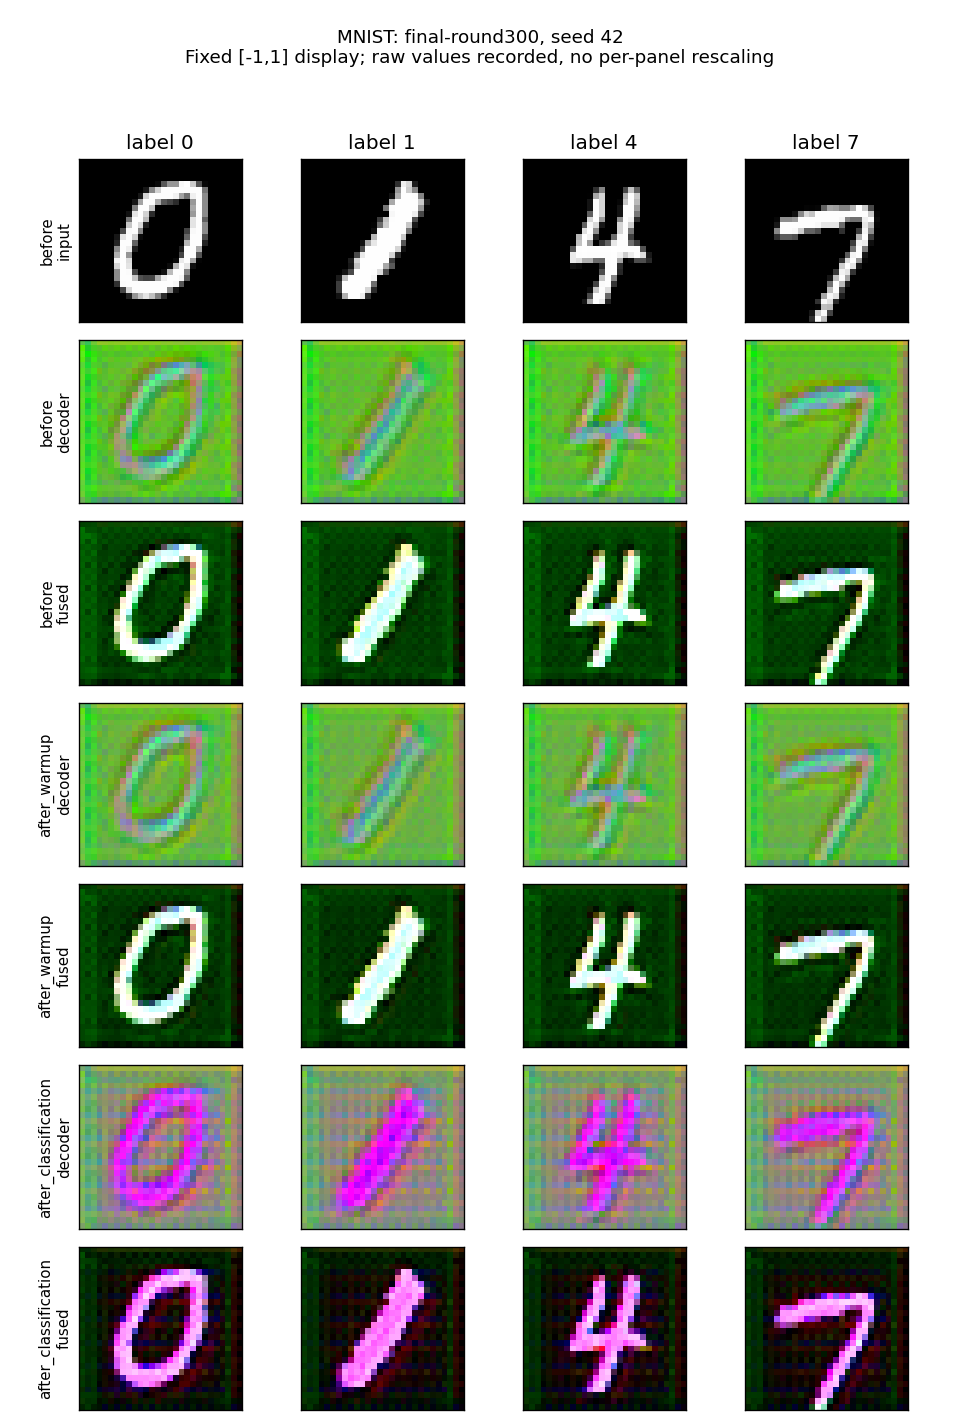
\includegraphics[width=.56in,trim=47.4bp 663.0bp 430.2bp 95.4bp,clip]{figures/digits/final-round300-MNIST.png} & 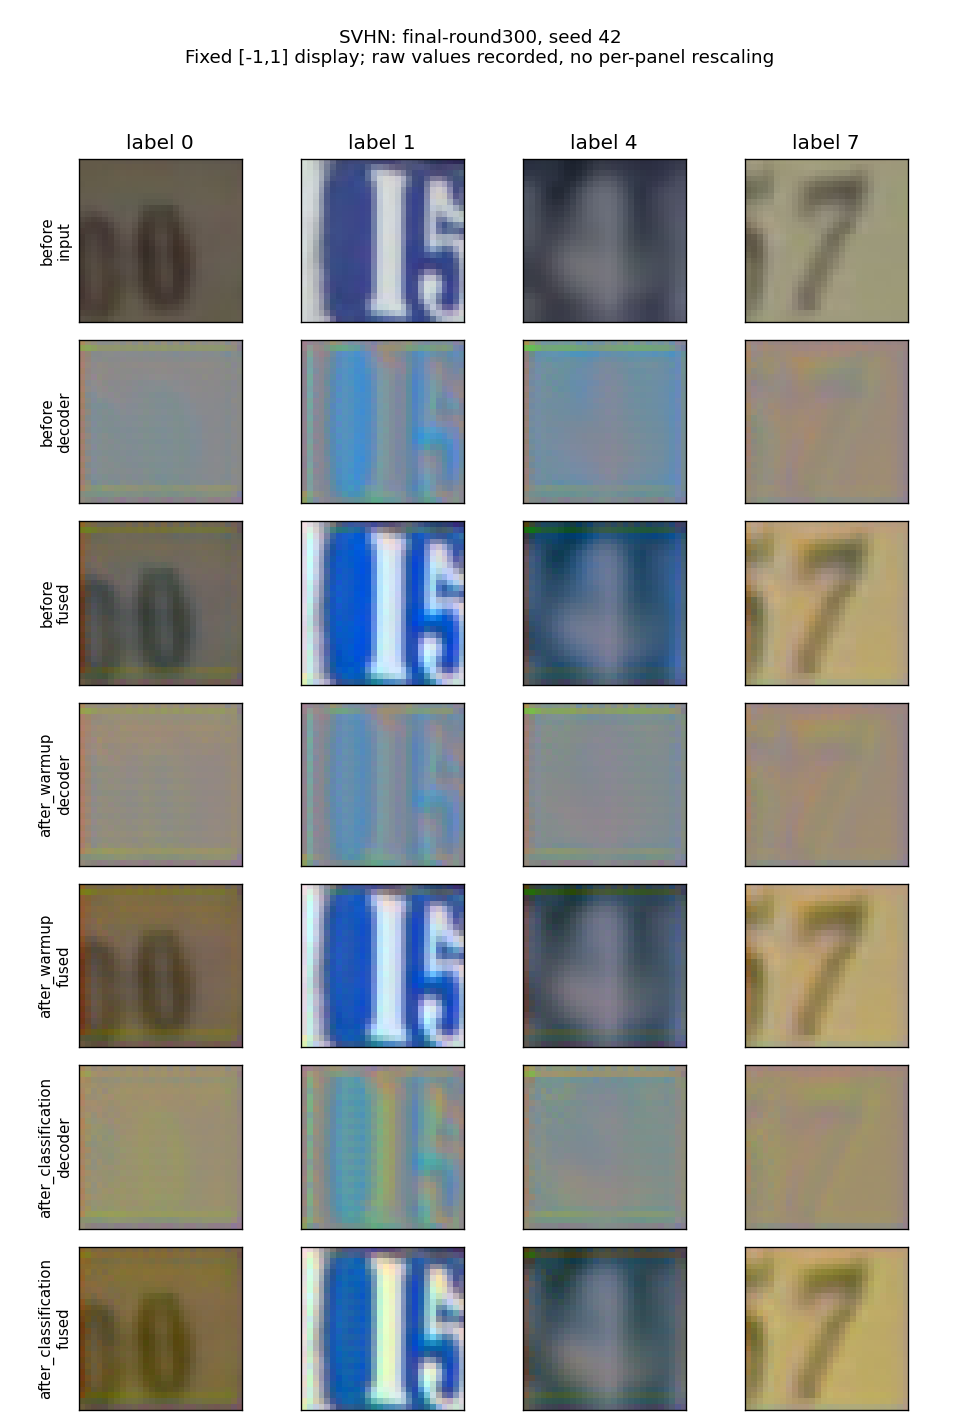
\includegraphics[width=.56in,trim=47.4bp 663.0bp 430.2bp 95.4bp,clip]{figures/digits/final-round300-SVHN.png} & 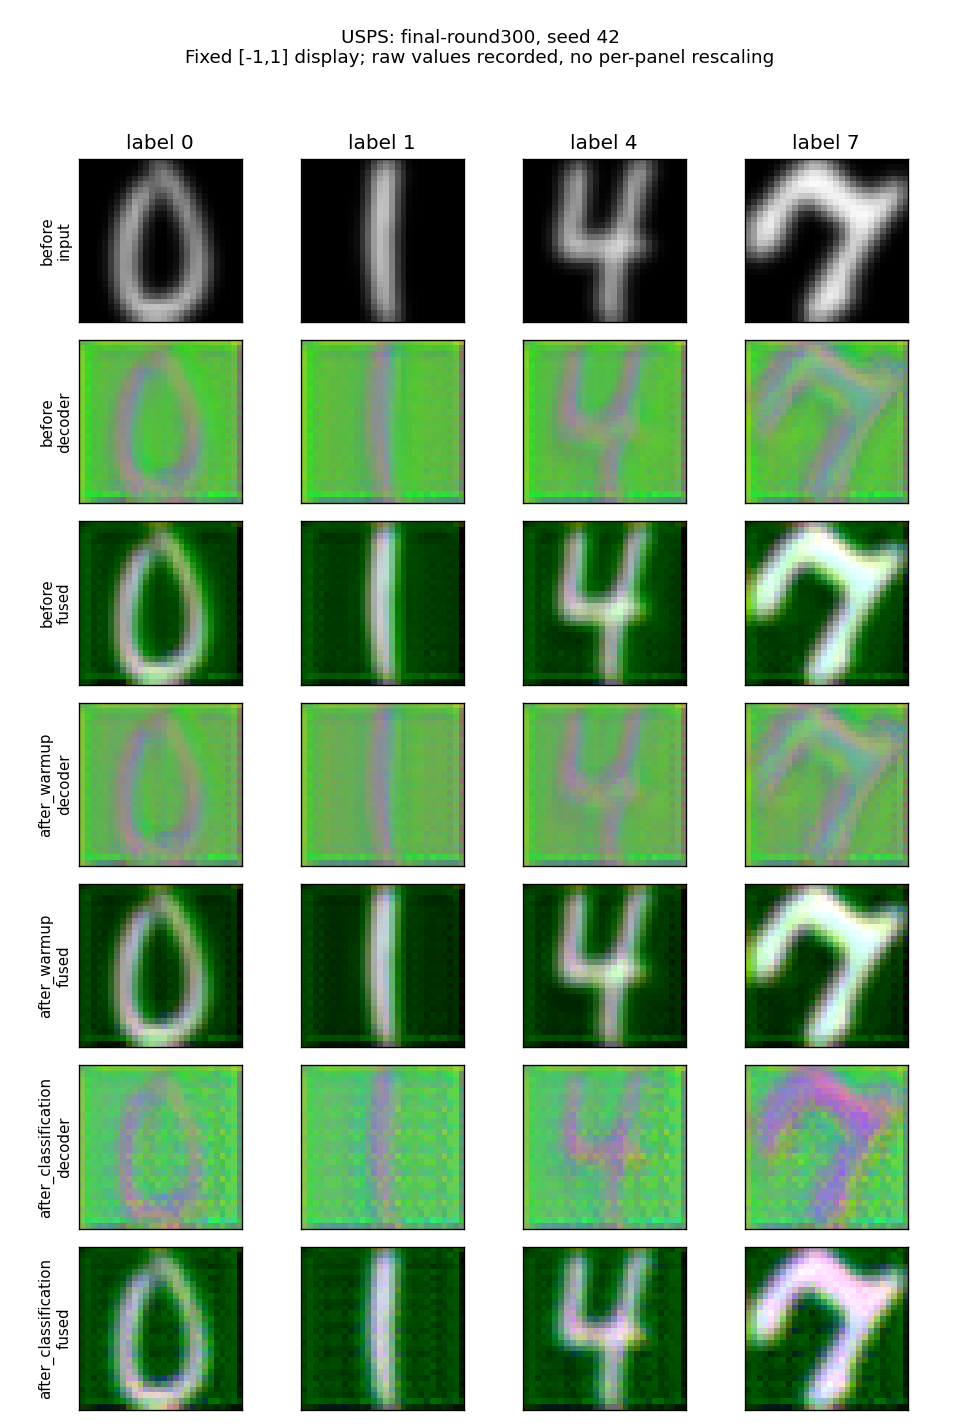
\includegraphics[width=.56in,trim=47.4bp 663.0bp 430.2bp 95.4bp,clip]{figures/digits/final-round300-USPS.png} & 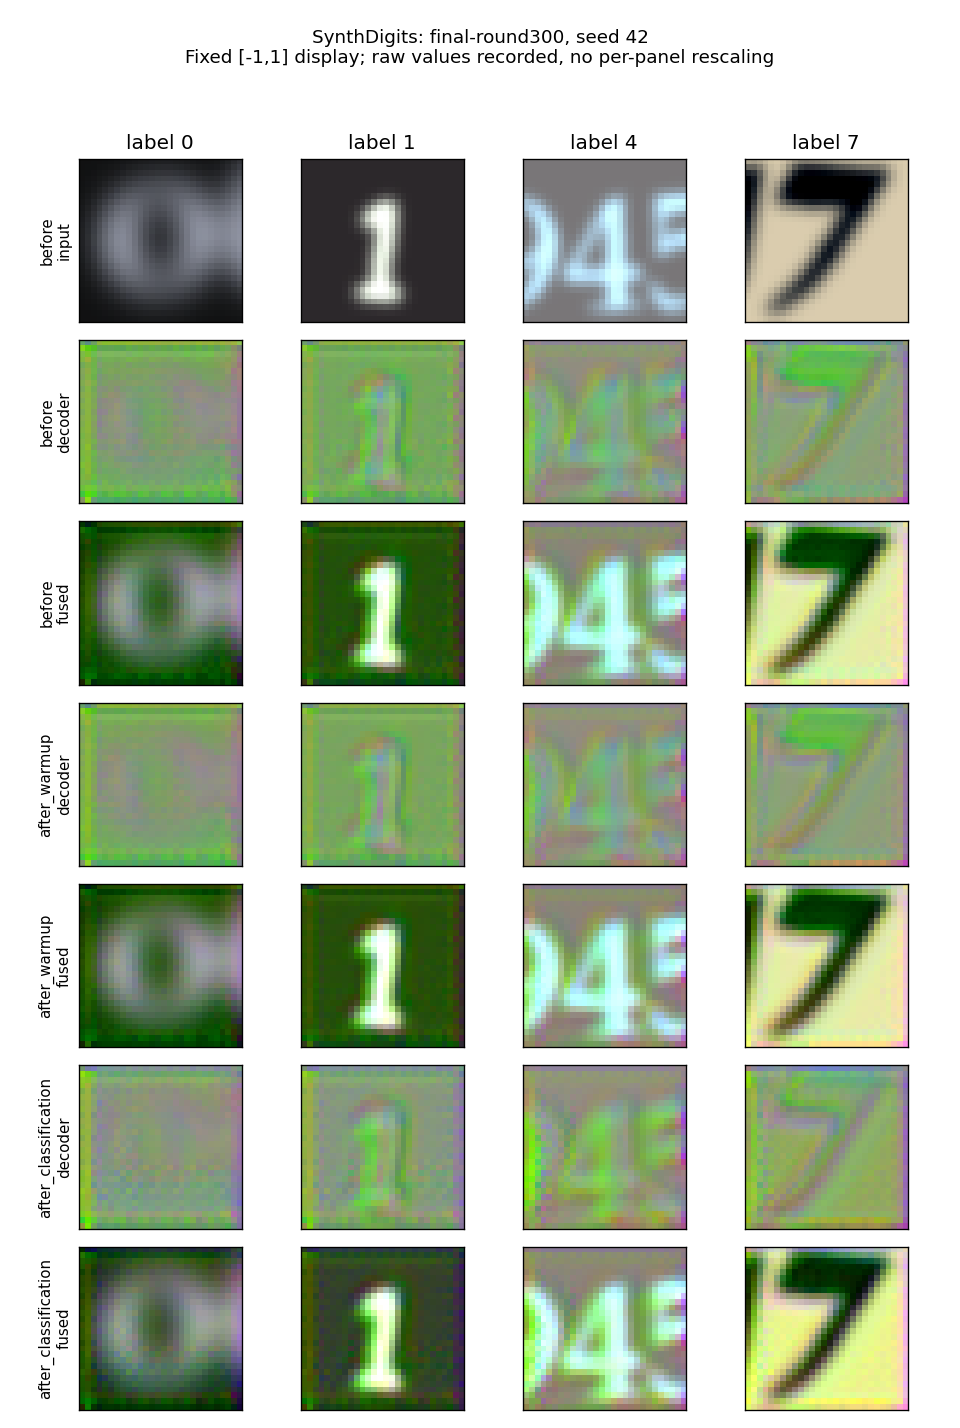
\includegraphics[width=.56in,trim=47.4bp 663.0bp 430.2bp 95.4bp,clip]{figures/digits/final-round300-SynthDigits.png} & 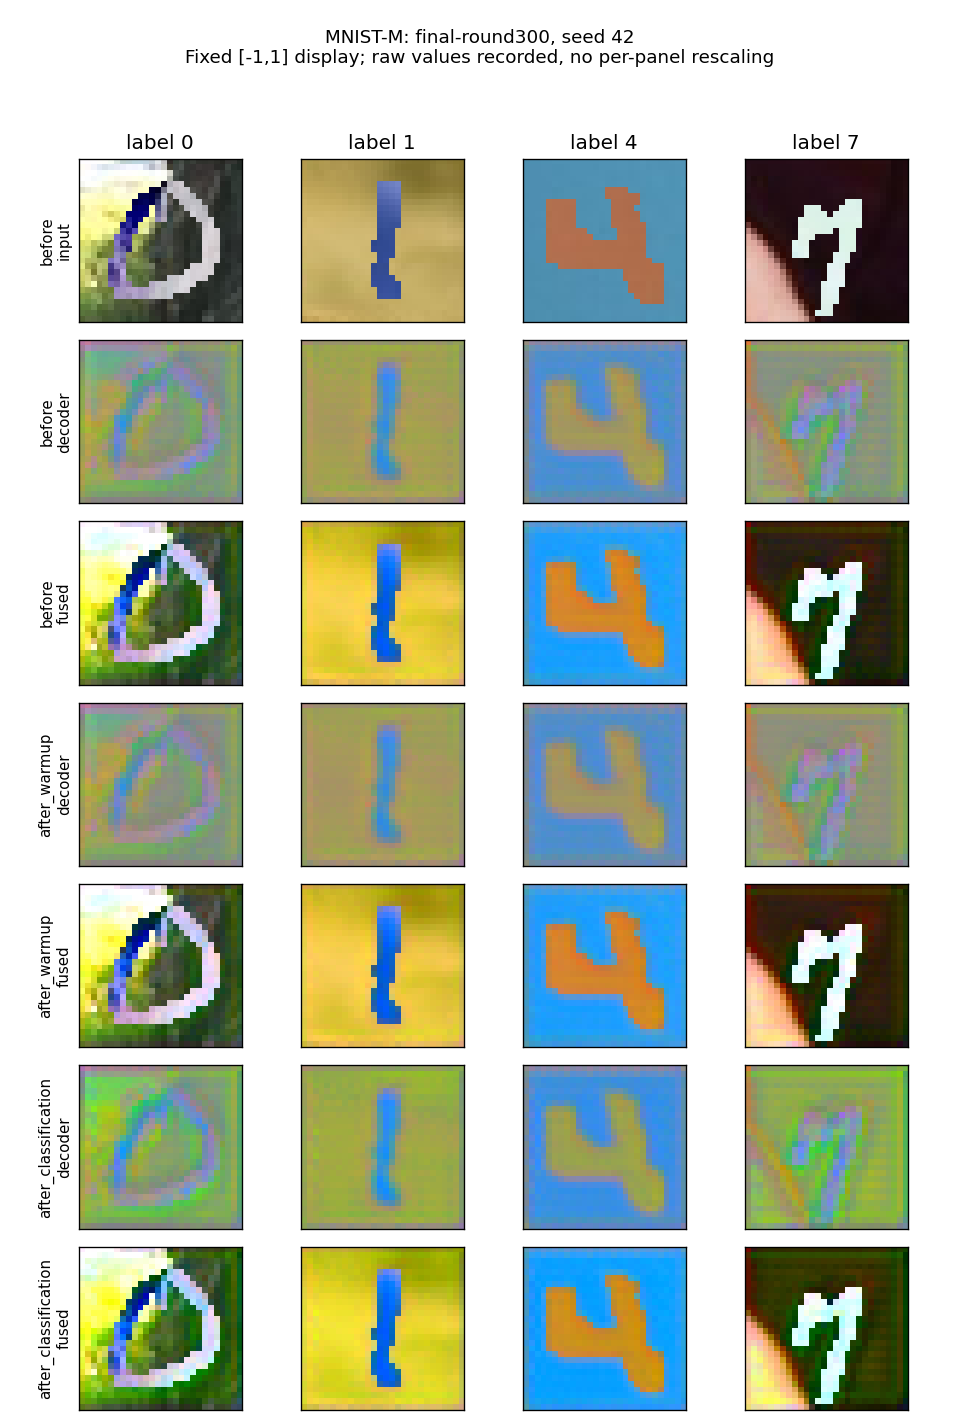
\includegraphics[width=.56in,trim=47.4bp 663.0bp 430.2bp 95.4bp,clip]{figures/digits/final-round300-MNIST-M.png} \\[-2pt]
\raisebox{.20in}{\scriptsize\shortstack[r]{Before\\decoder}} & 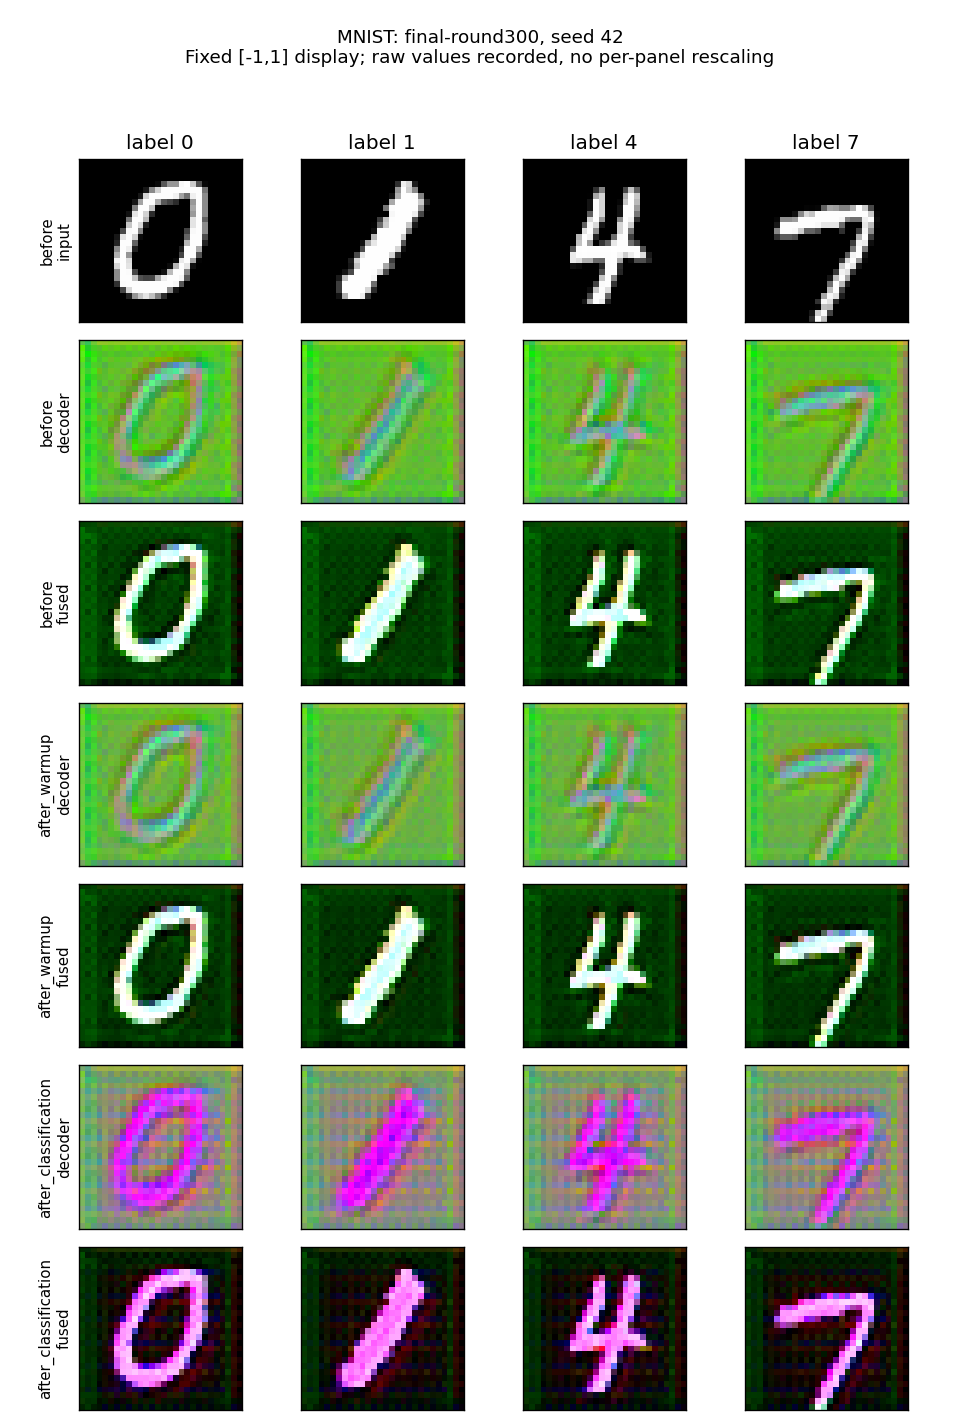
\includegraphics[width=.56in,trim=47.4bp 554.4bp 430.2bp 204.0bp,clip]{figures/digits/final-round300-MNIST.png} & 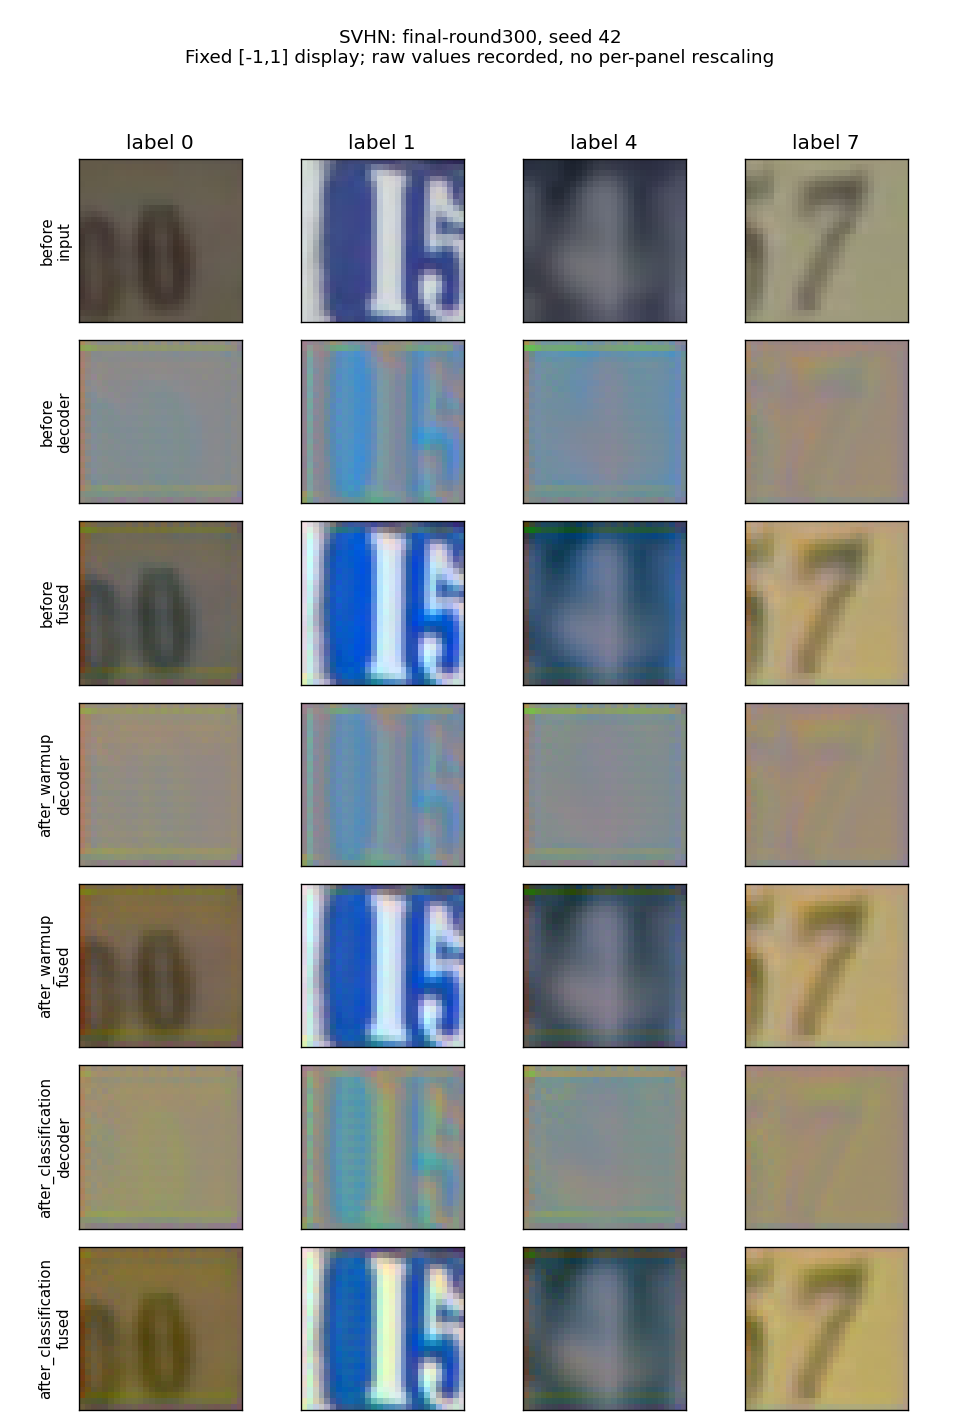
\includegraphics[width=.56in,trim=47.4bp 554.4bp 430.2bp 204.0bp,clip]{figures/digits/final-round300-SVHN.png} & 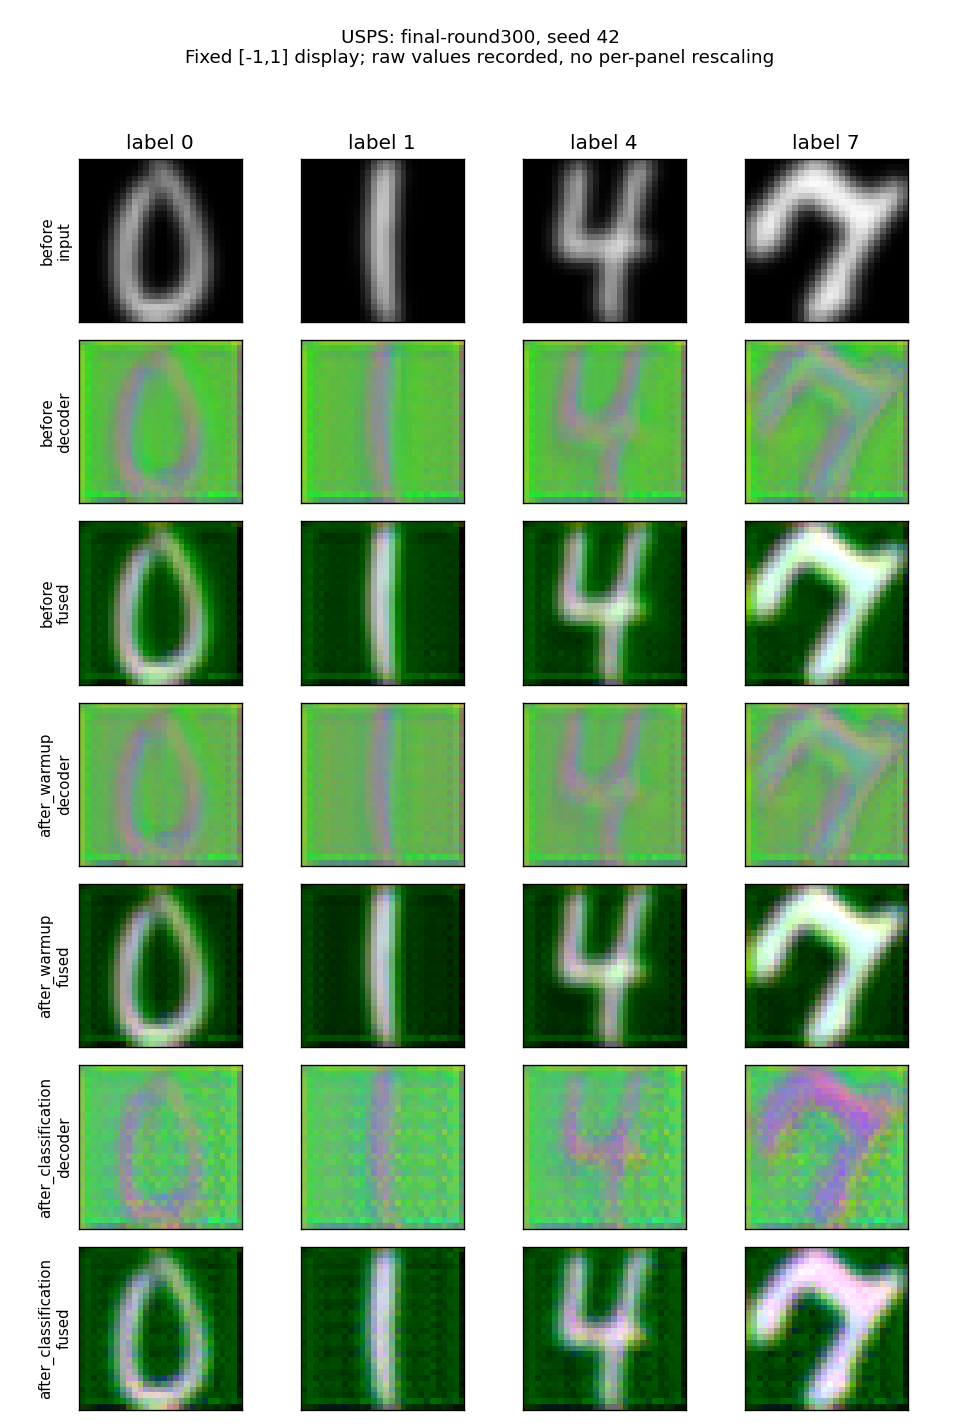
\includegraphics[width=.56in,trim=47.4bp 554.4bp 430.2bp 204.0bp,clip]{figures/digits/final-round300-USPS.png} & 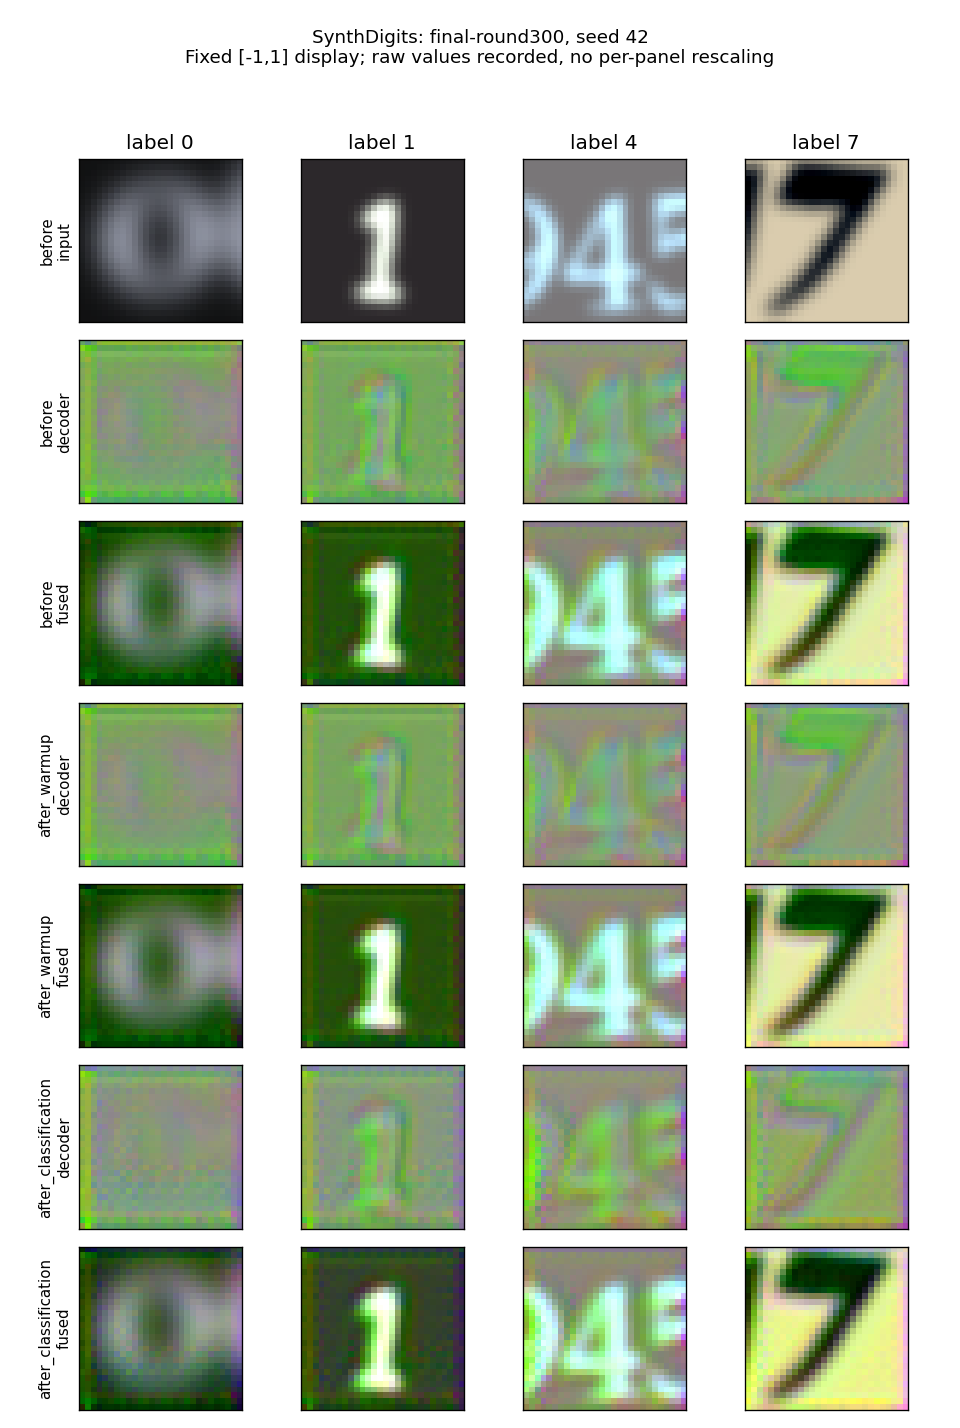
\includegraphics[width=.56in,trim=47.4bp 554.4bp 430.2bp 204.0bp,clip]{figures/digits/final-round300-SynthDigits.png} & 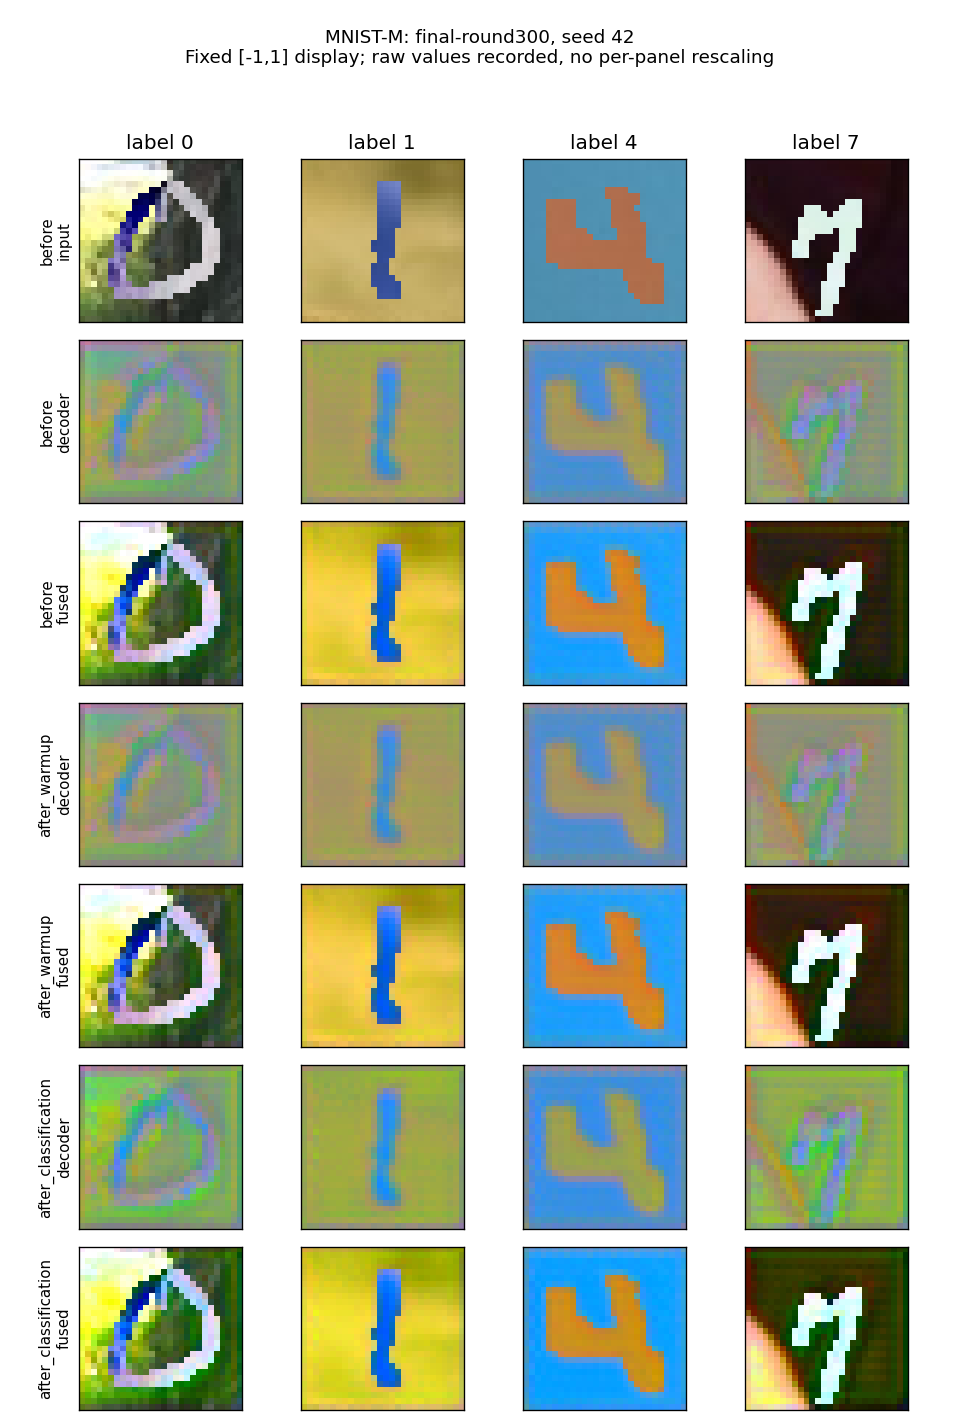
\includegraphics[width=.56in,trim=47.4bp 554.4bp 430.2bp 204.0bp,clip]{figures/digits/final-round300-MNIST-M.png} \\[-2pt]
\raisebox{.20in}{\scriptsize\shortstack[r]{Before\\fused}} & 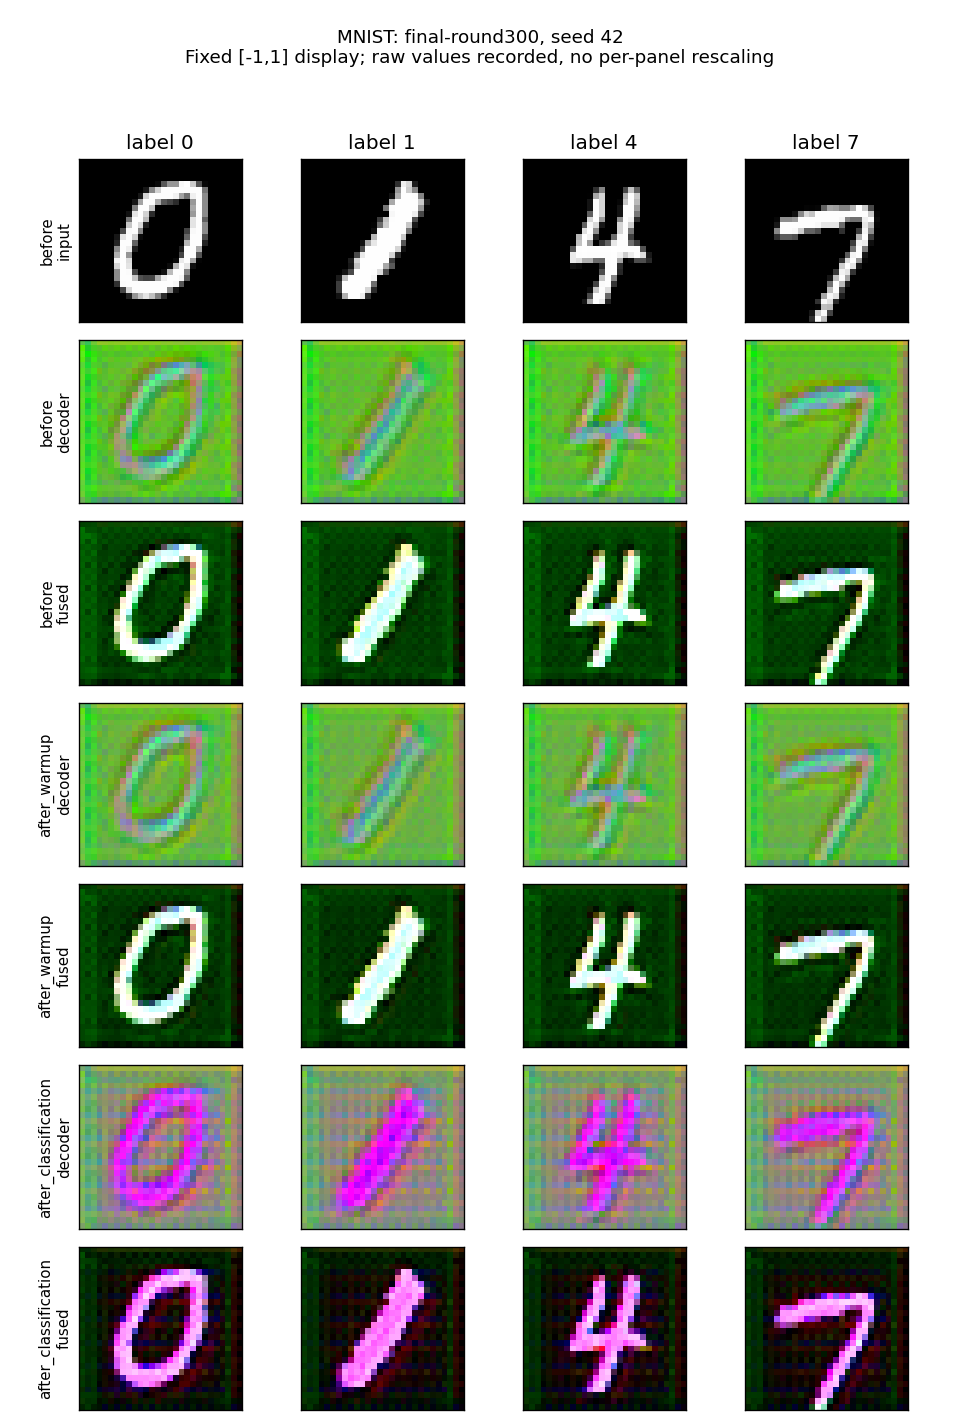
\includegraphics[width=.56in,trim=47.4bp 445.2bp 430.2bp 313.2bp,clip]{figures/digits/final-round300-MNIST.png} & 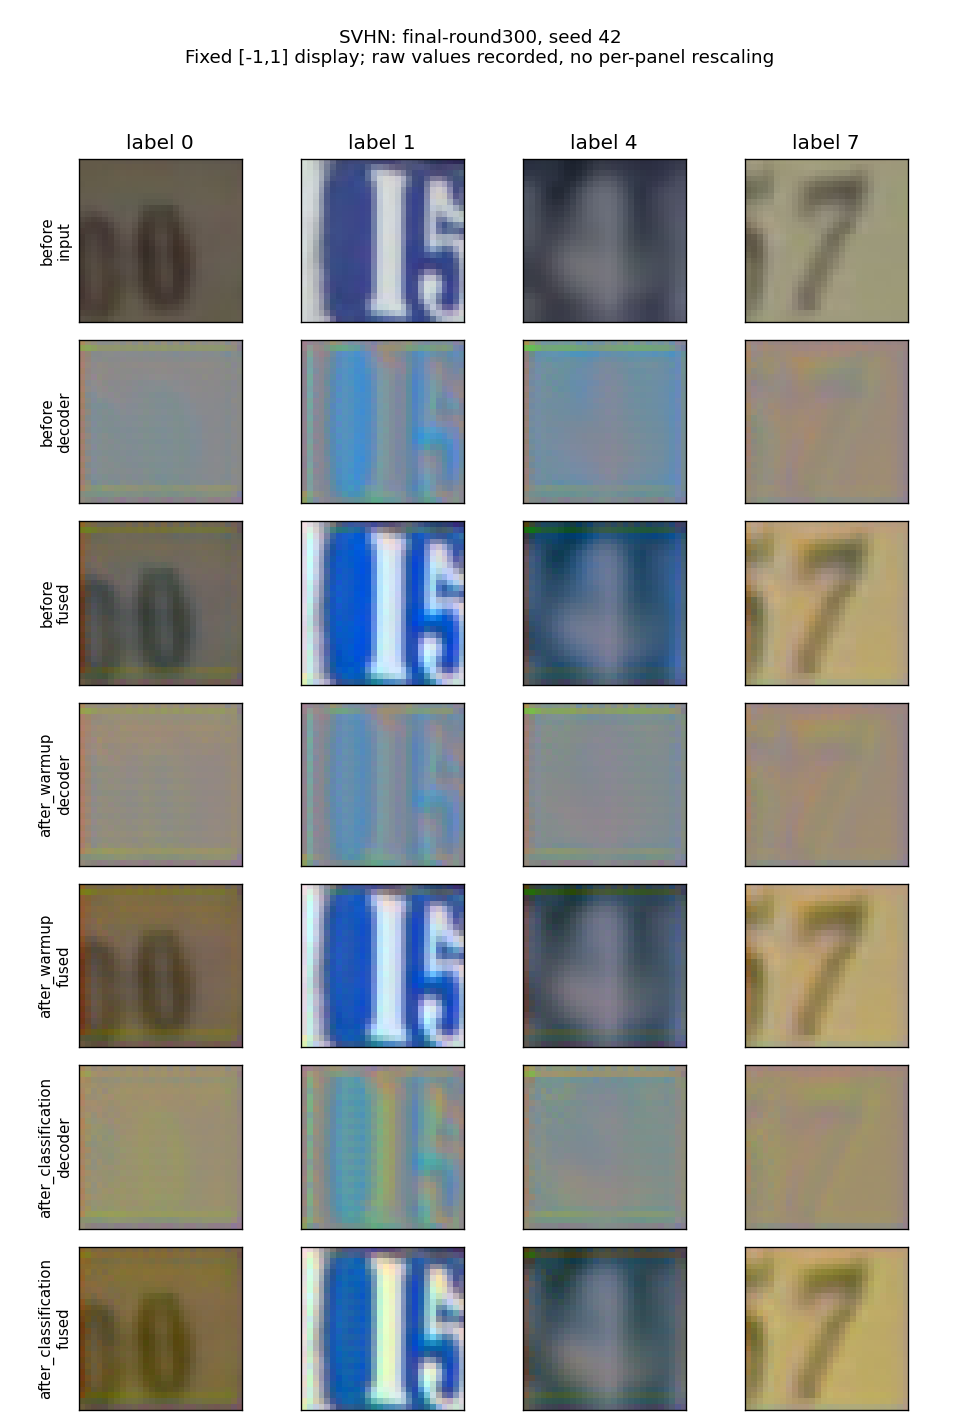
\includegraphics[width=.56in,trim=47.4bp 445.2bp 430.2bp 313.2bp,clip]{figures/digits/final-round300-SVHN.png} & 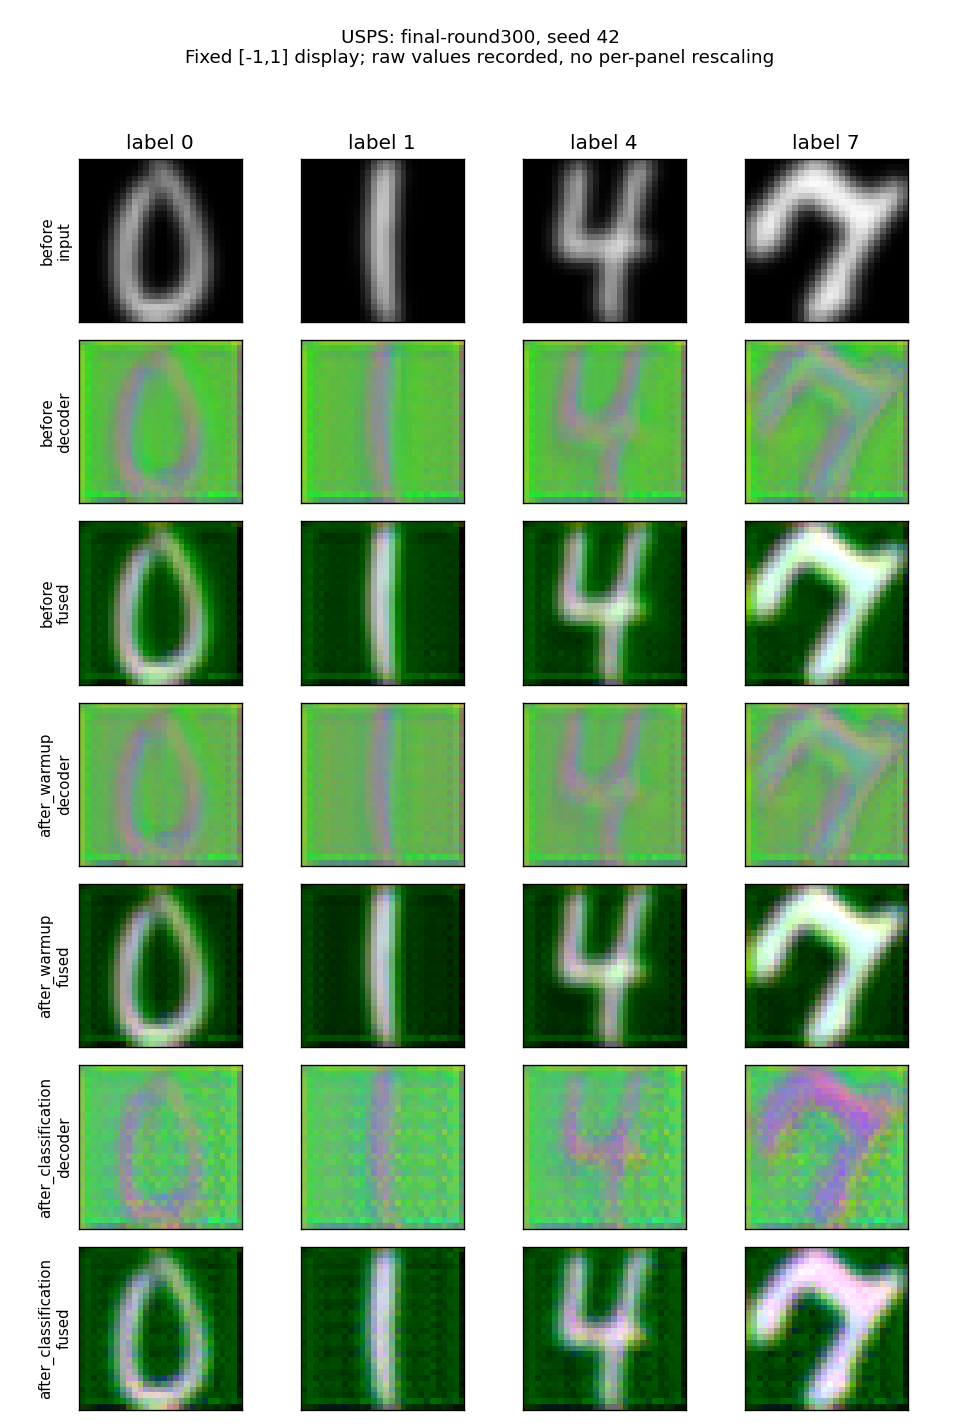
\includegraphics[width=.56in,trim=47.4bp 445.2bp 430.2bp 313.2bp,clip]{figures/digits/final-round300-USPS.png} & 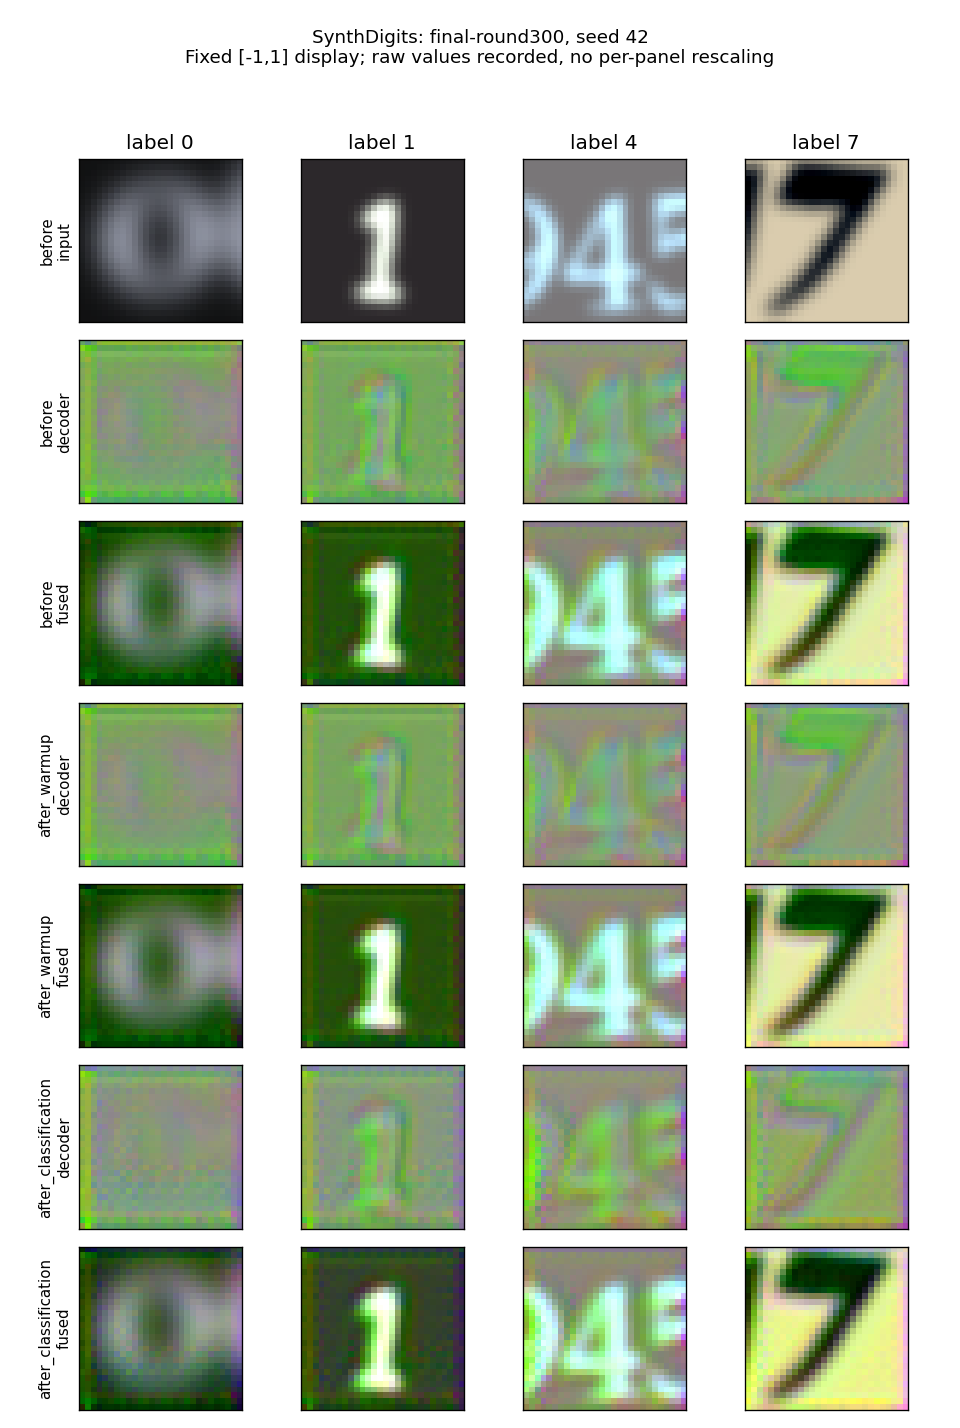
\includegraphics[width=.56in,trim=47.4bp 445.2bp 430.2bp 313.2bp,clip]{figures/digits/final-round300-SynthDigits.png} & 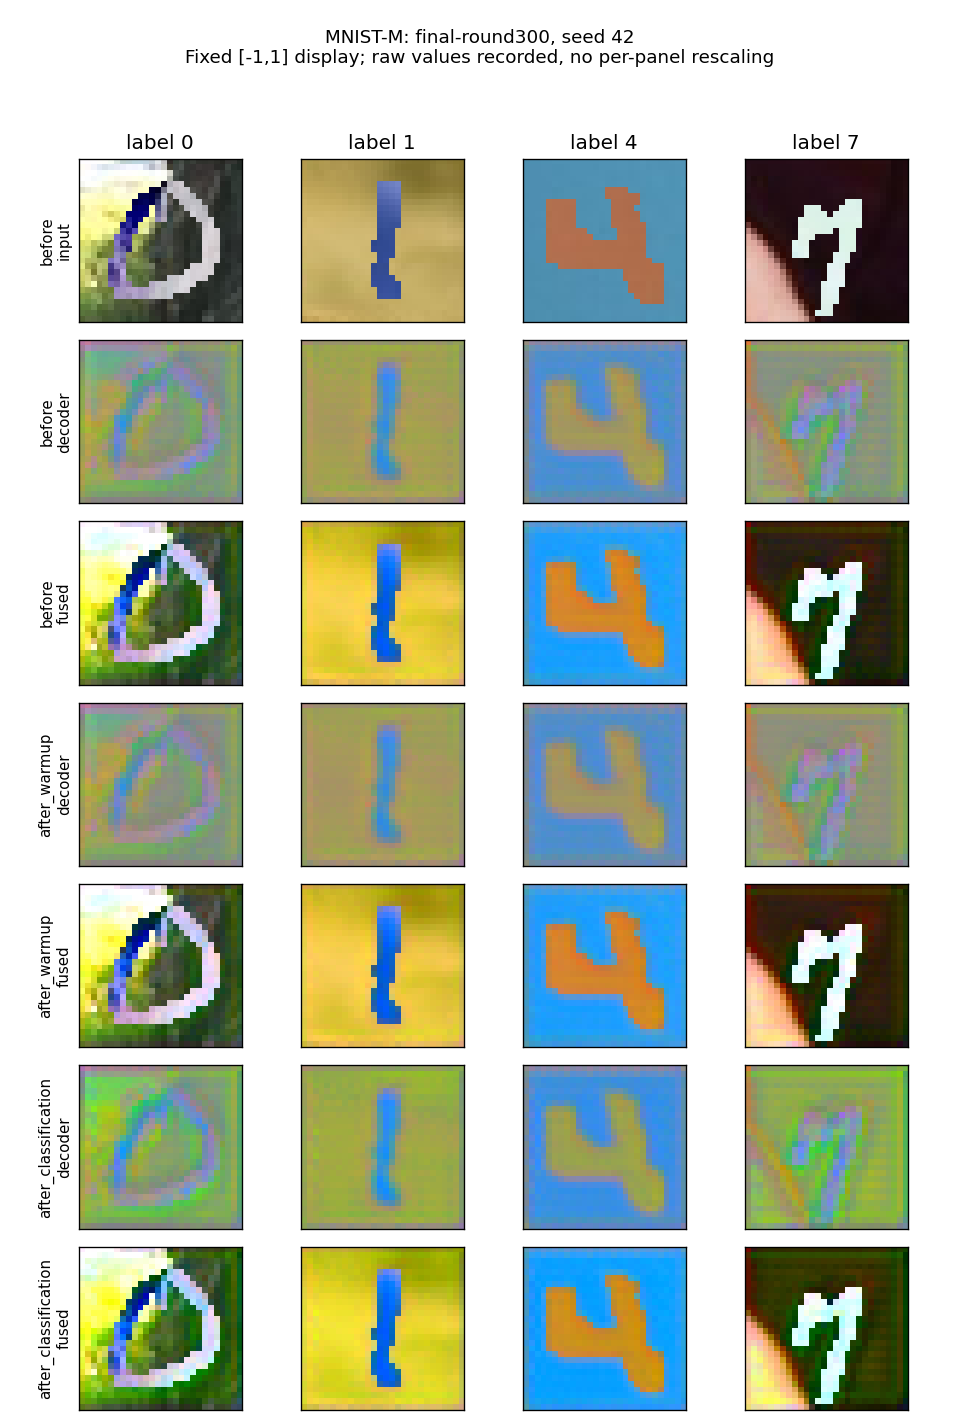
\includegraphics[width=.56in,trim=47.4bp 445.2bp 430.2bp 313.2bp,clip]{figures/digits/final-round300-MNIST-M.png} \\[-2pt]
\raisebox{.20in}{\scriptsize\shortstack[r]{After warm-up\\decoder}} & 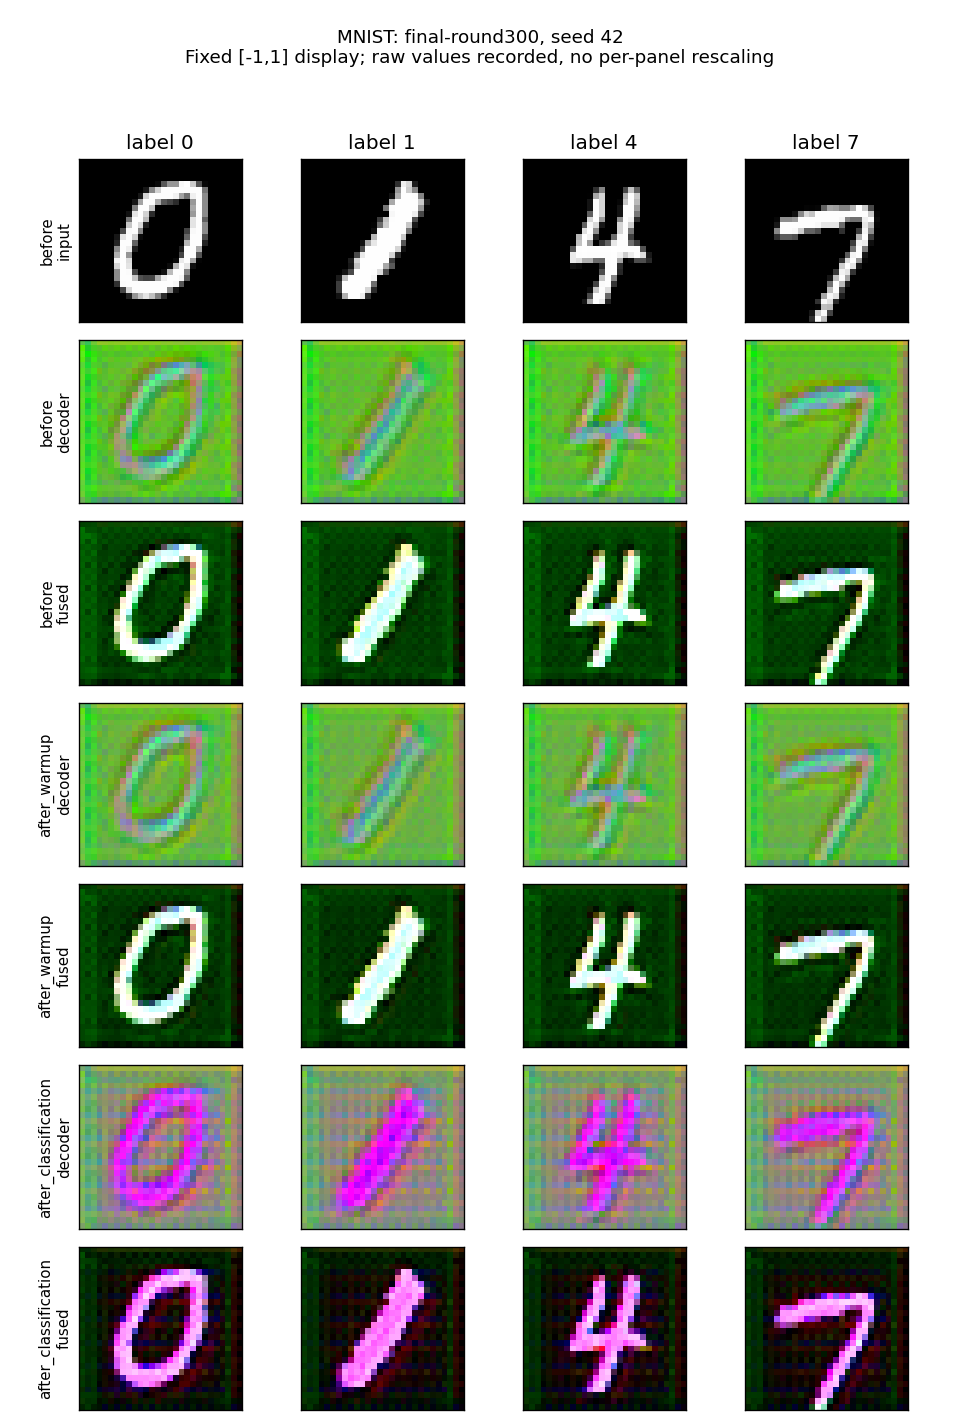
\includegraphics[width=.56in,trim=47.4bp 336.0bp 430.2bp 422.4bp,clip]{figures/digits/final-round300-MNIST.png} & 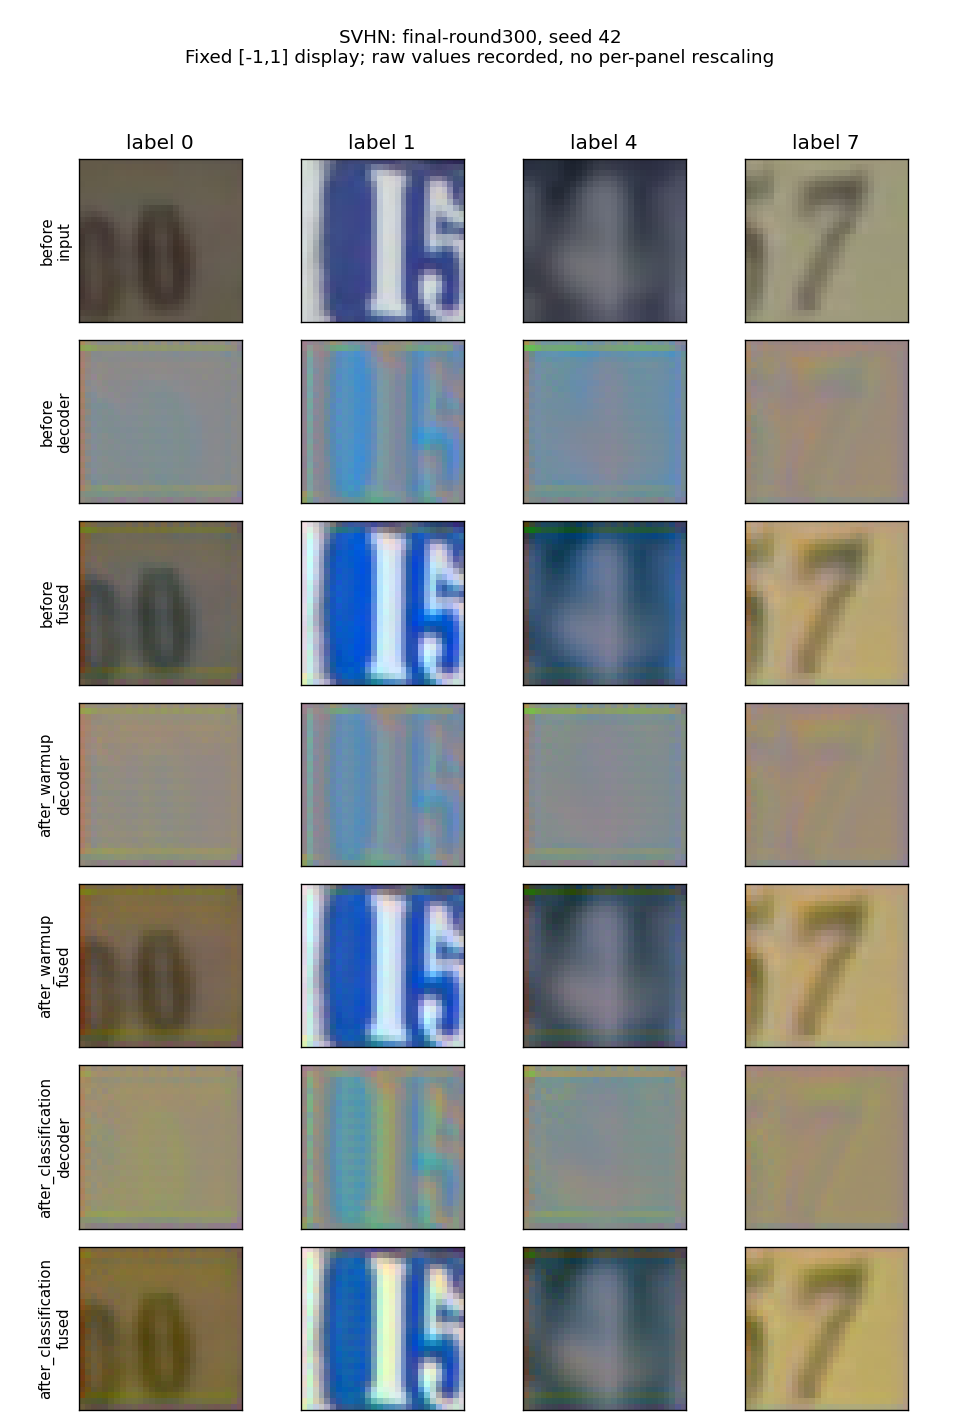
\includegraphics[width=.56in,trim=47.4bp 336.0bp 430.2bp 422.4bp,clip]{figures/digits/final-round300-SVHN.png} & 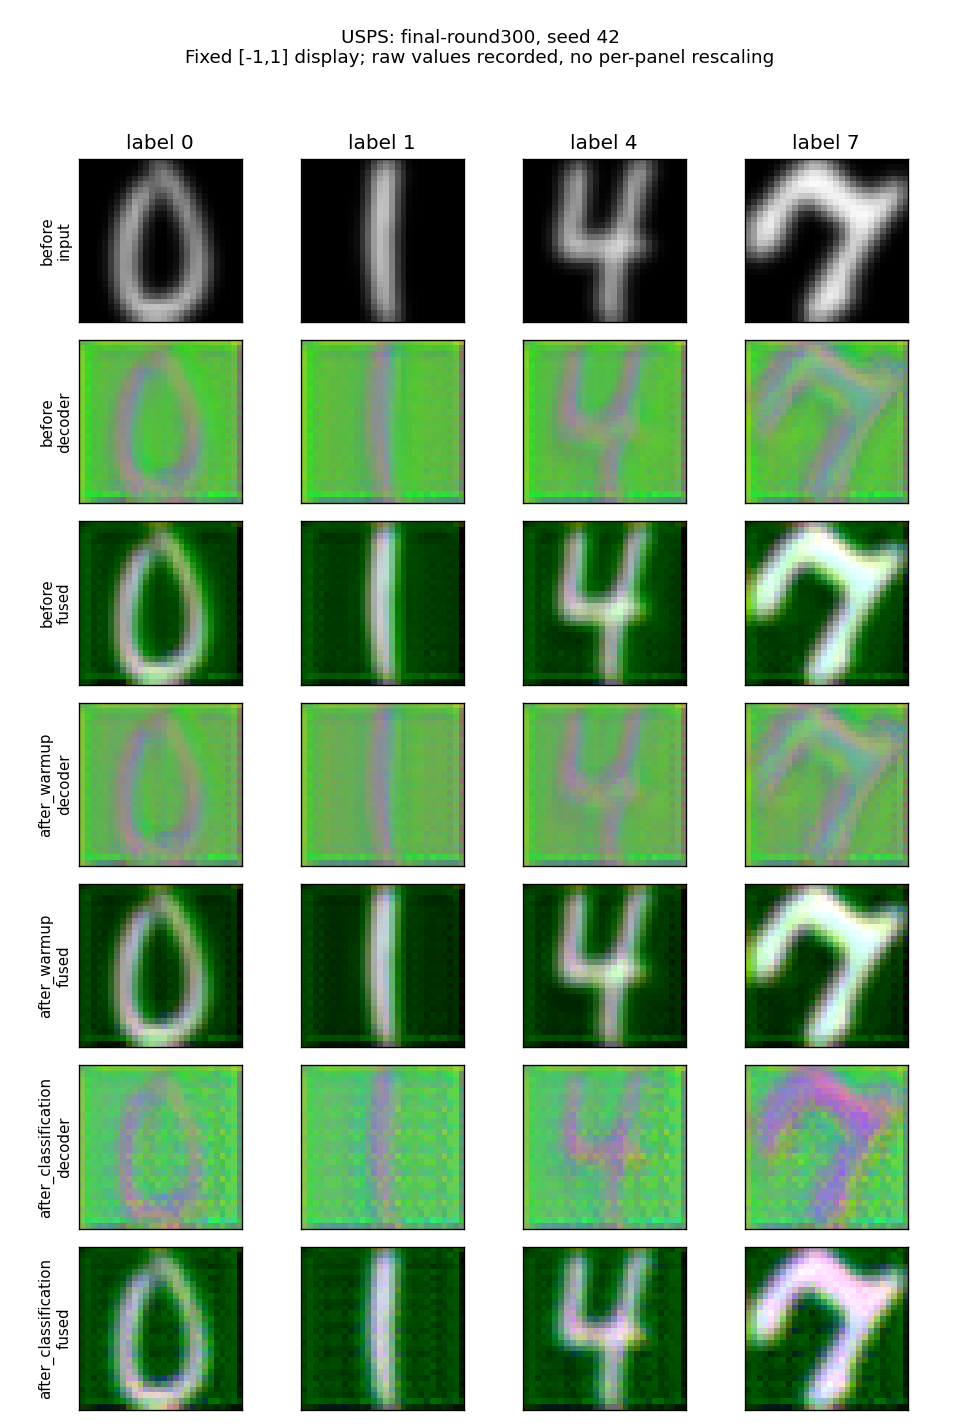
\includegraphics[width=.56in,trim=47.4bp 336.0bp 430.2bp 422.4bp,clip]{figures/digits/final-round300-USPS.png} & 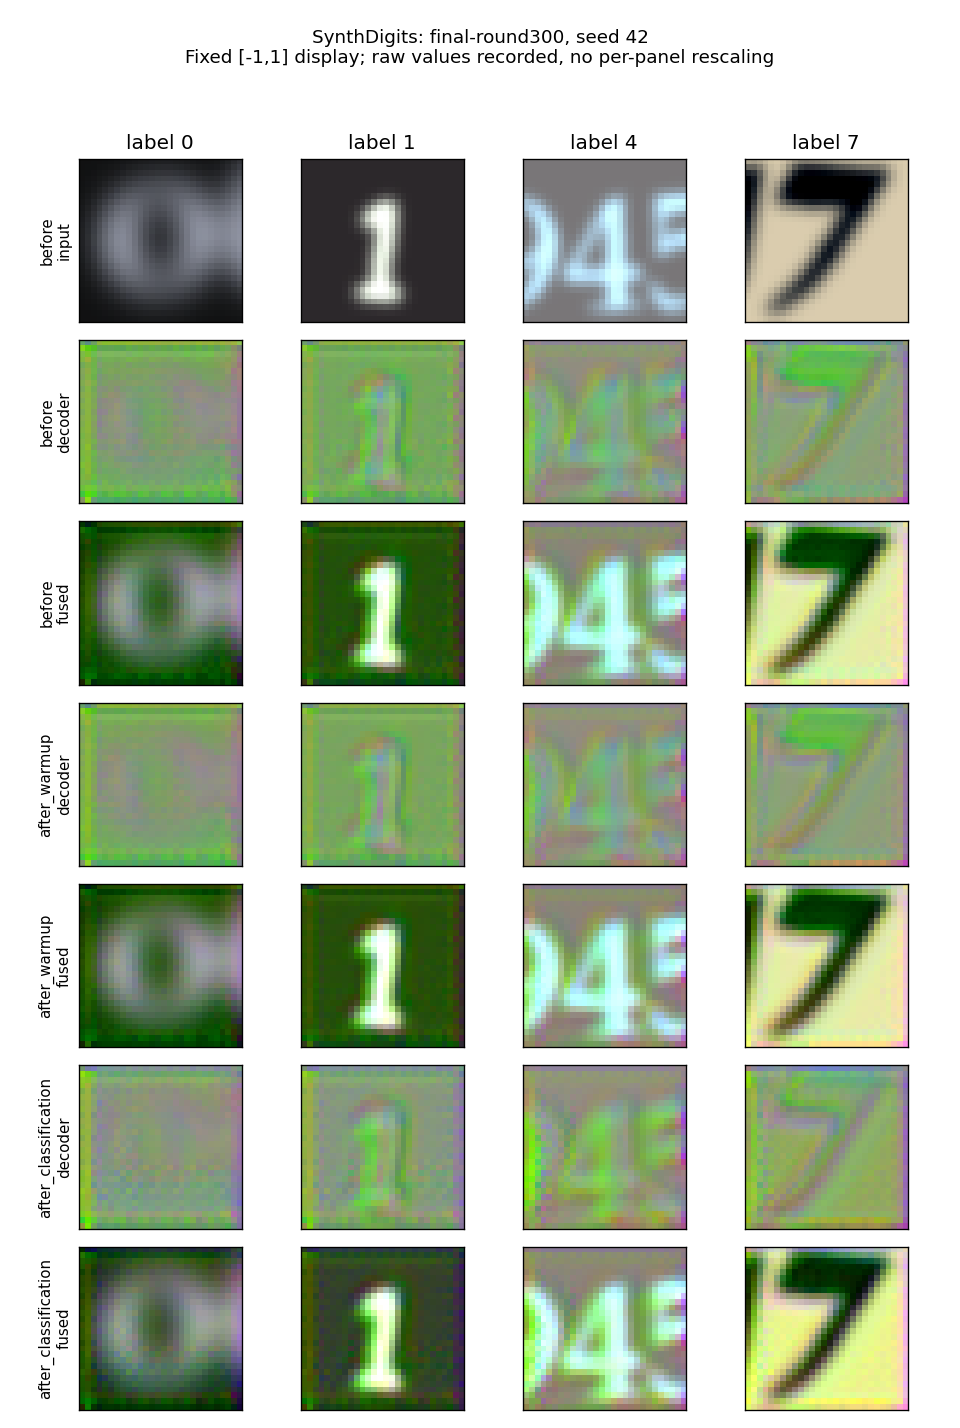
\includegraphics[width=.56in,trim=47.4bp 336.0bp 430.2bp 422.4bp,clip]{figures/digits/final-round300-SynthDigits.png} & 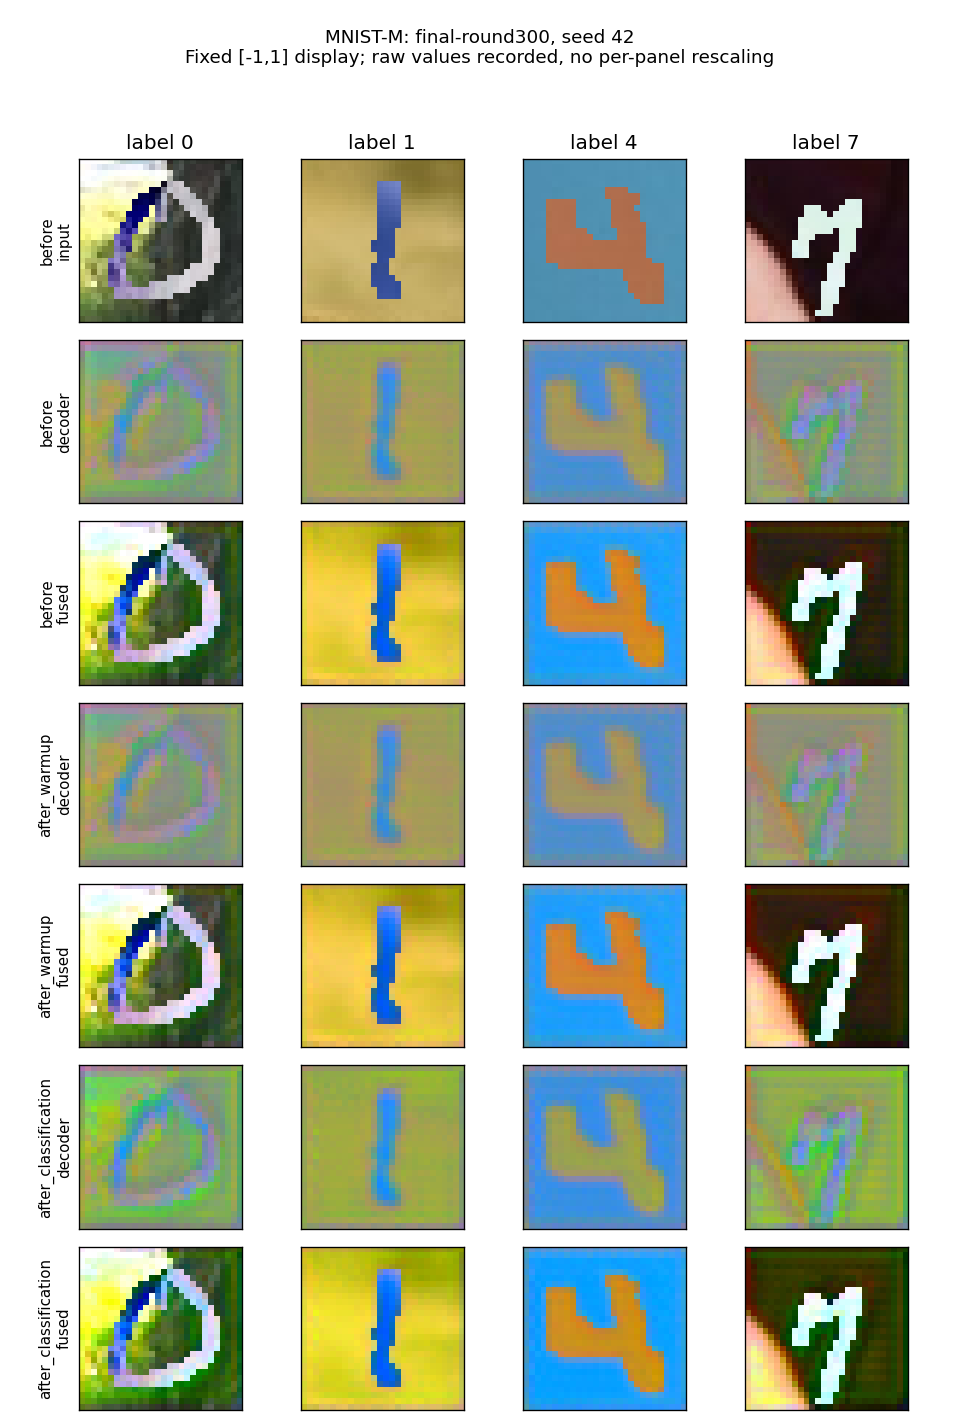
\includegraphics[width=.56in,trim=47.4bp 336.0bp 430.2bp 422.4bp,clip]{figures/digits/final-round300-MNIST-M.png} \\[-2pt]
\raisebox{.20in}{\scriptsize\shortstack[r]{After warm-up\\fused}} & 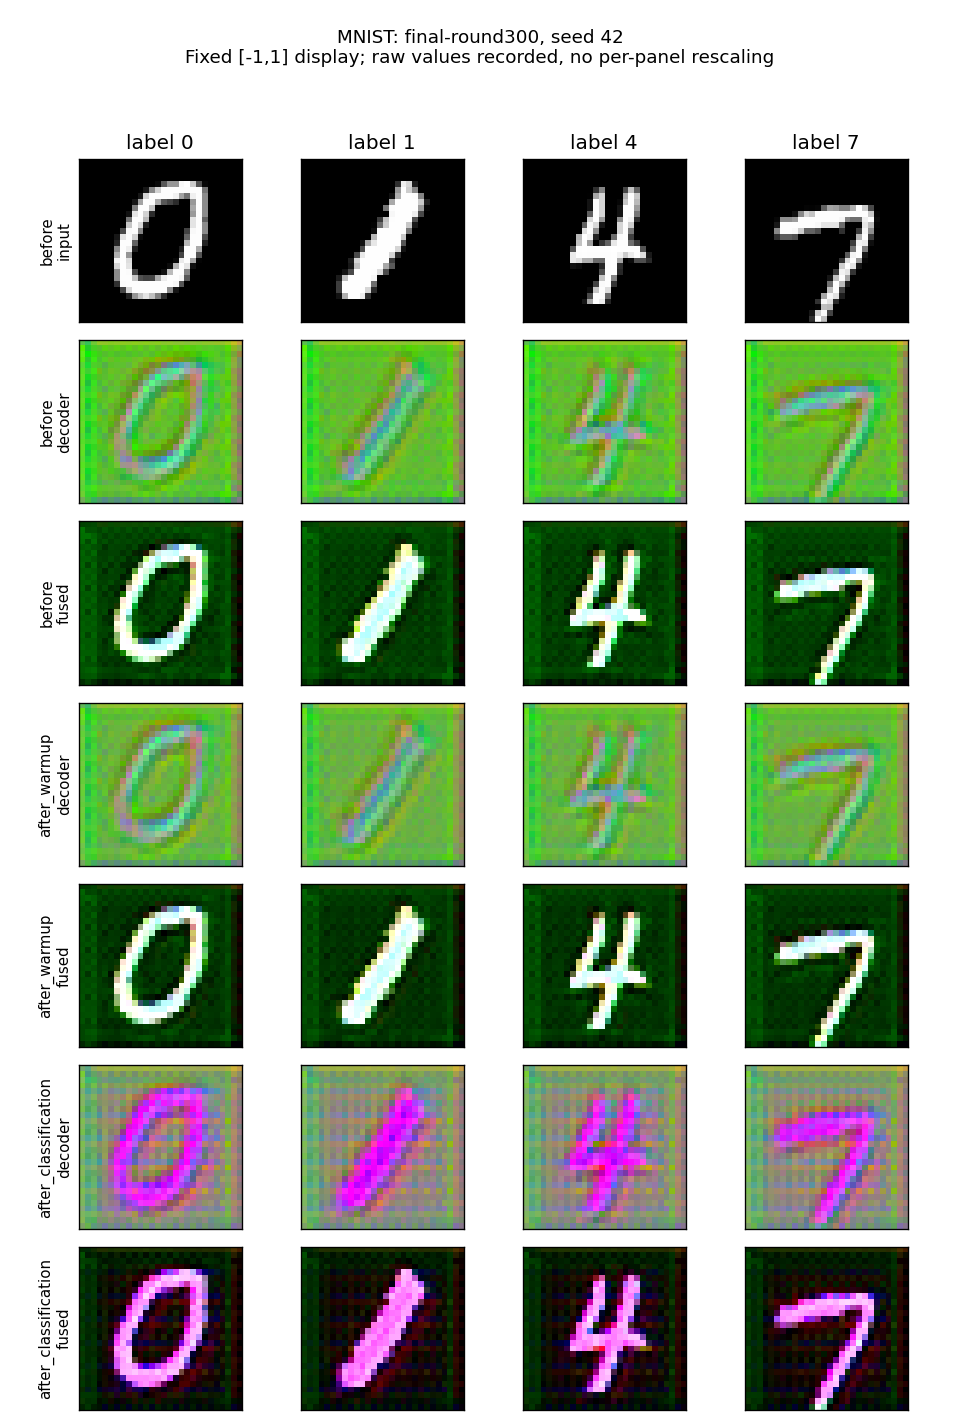
\includegraphics[width=.56in,trim=47.4bp 227.4bp 430.2bp 531.0bp,clip]{figures/digits/final-round300-MNIST.png} & 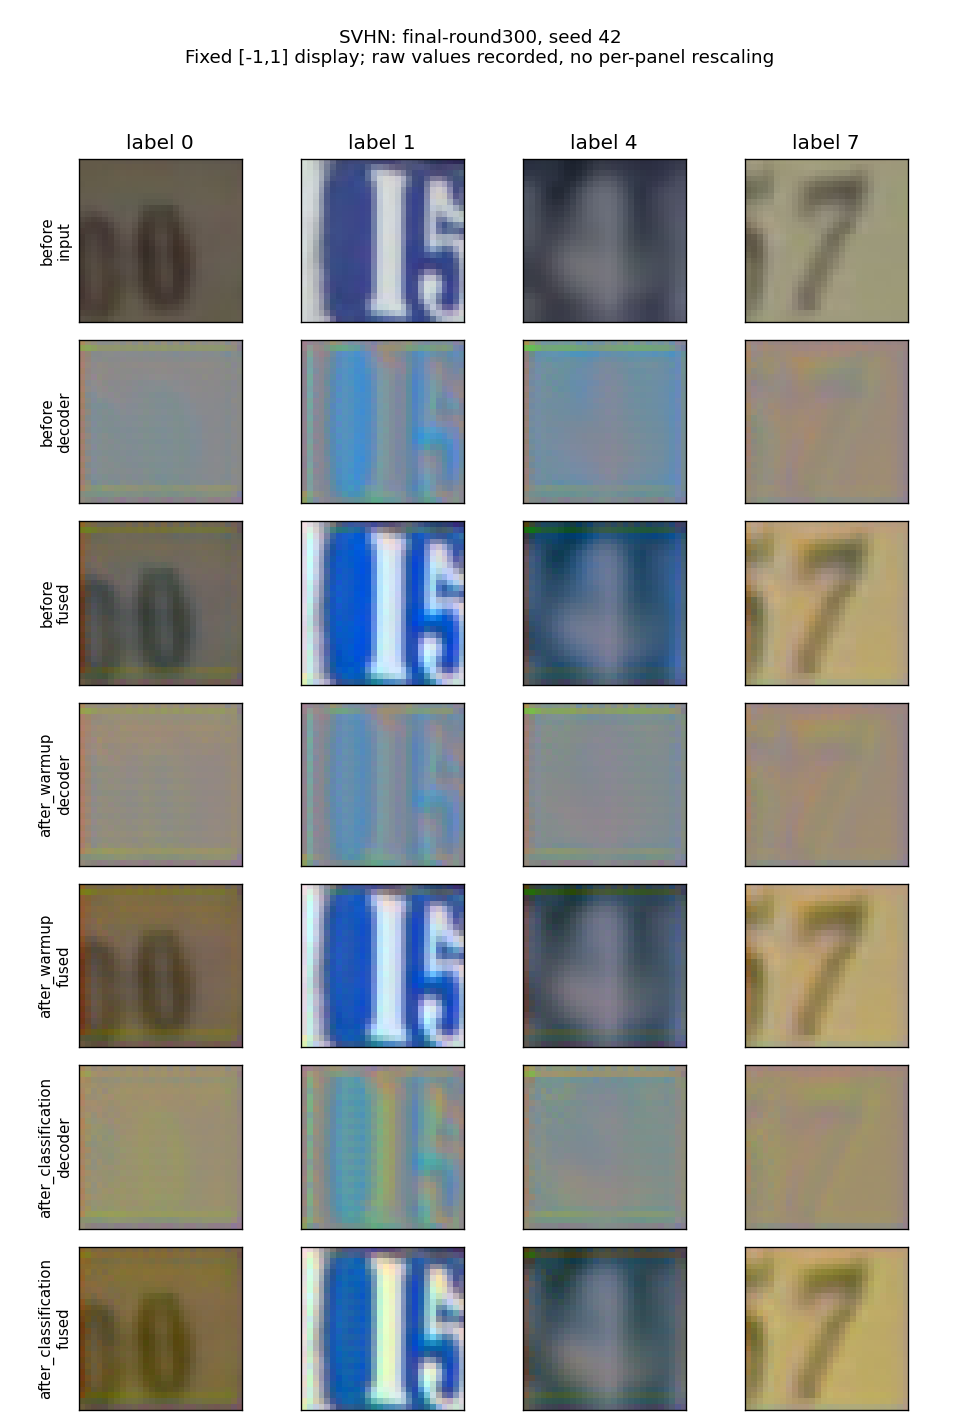
\includegraphics[width=.56in,trim=47.4bp 227.4bp 430.2bp 531.0bp,clip]{figures/digits/final-round300-SVHN.png} & 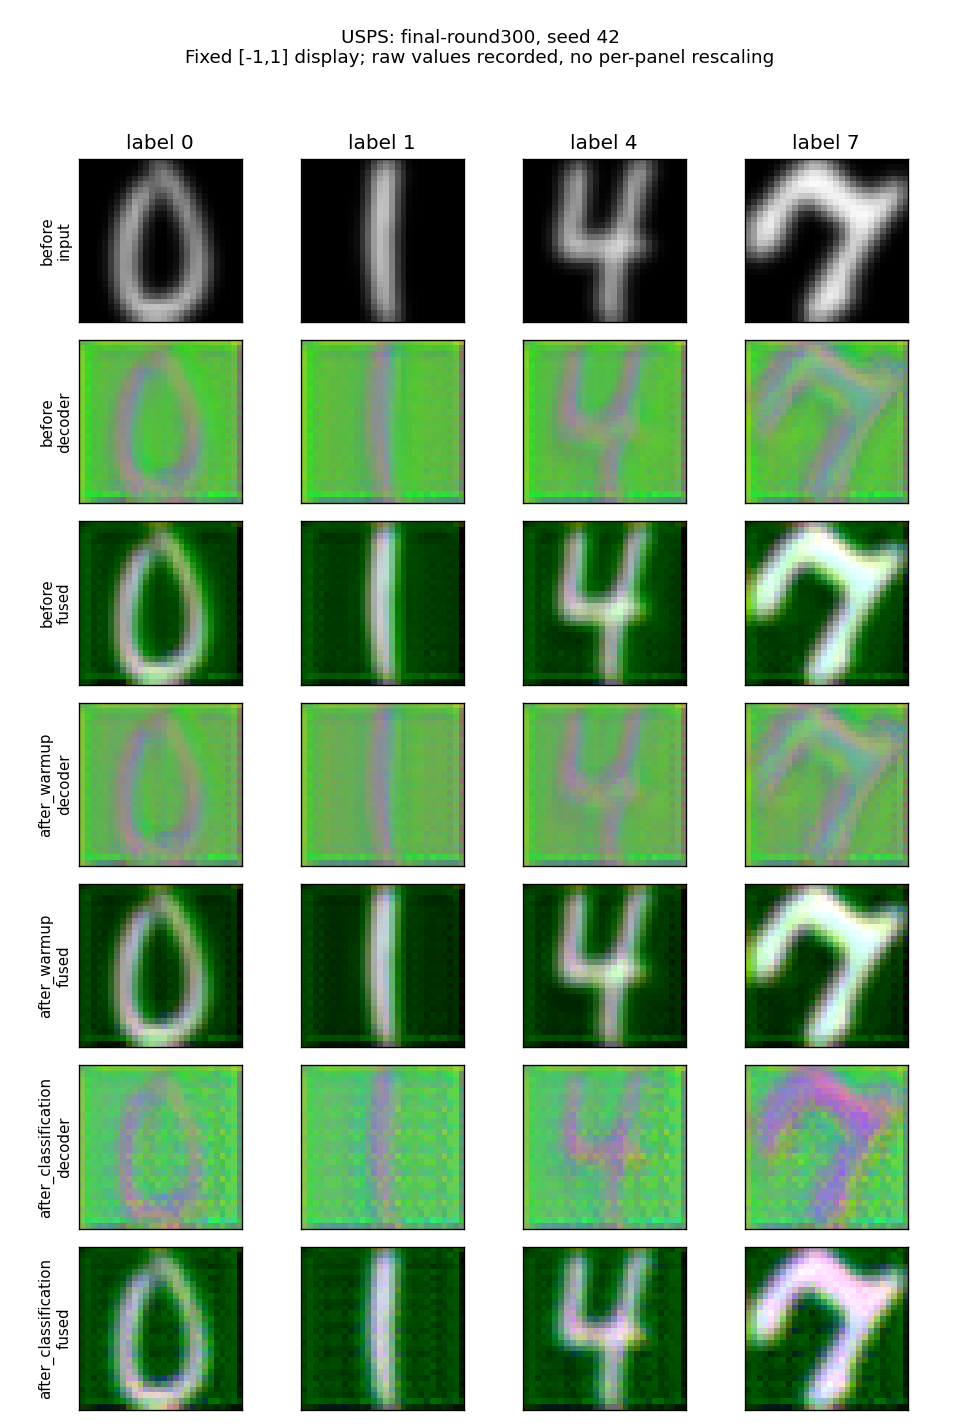
\includegraphics[width=.56in,trim=47.4bp 227.4bp 430.2bp 531.0bp,clip]{figures/digits/final-round300-USPS.png} & 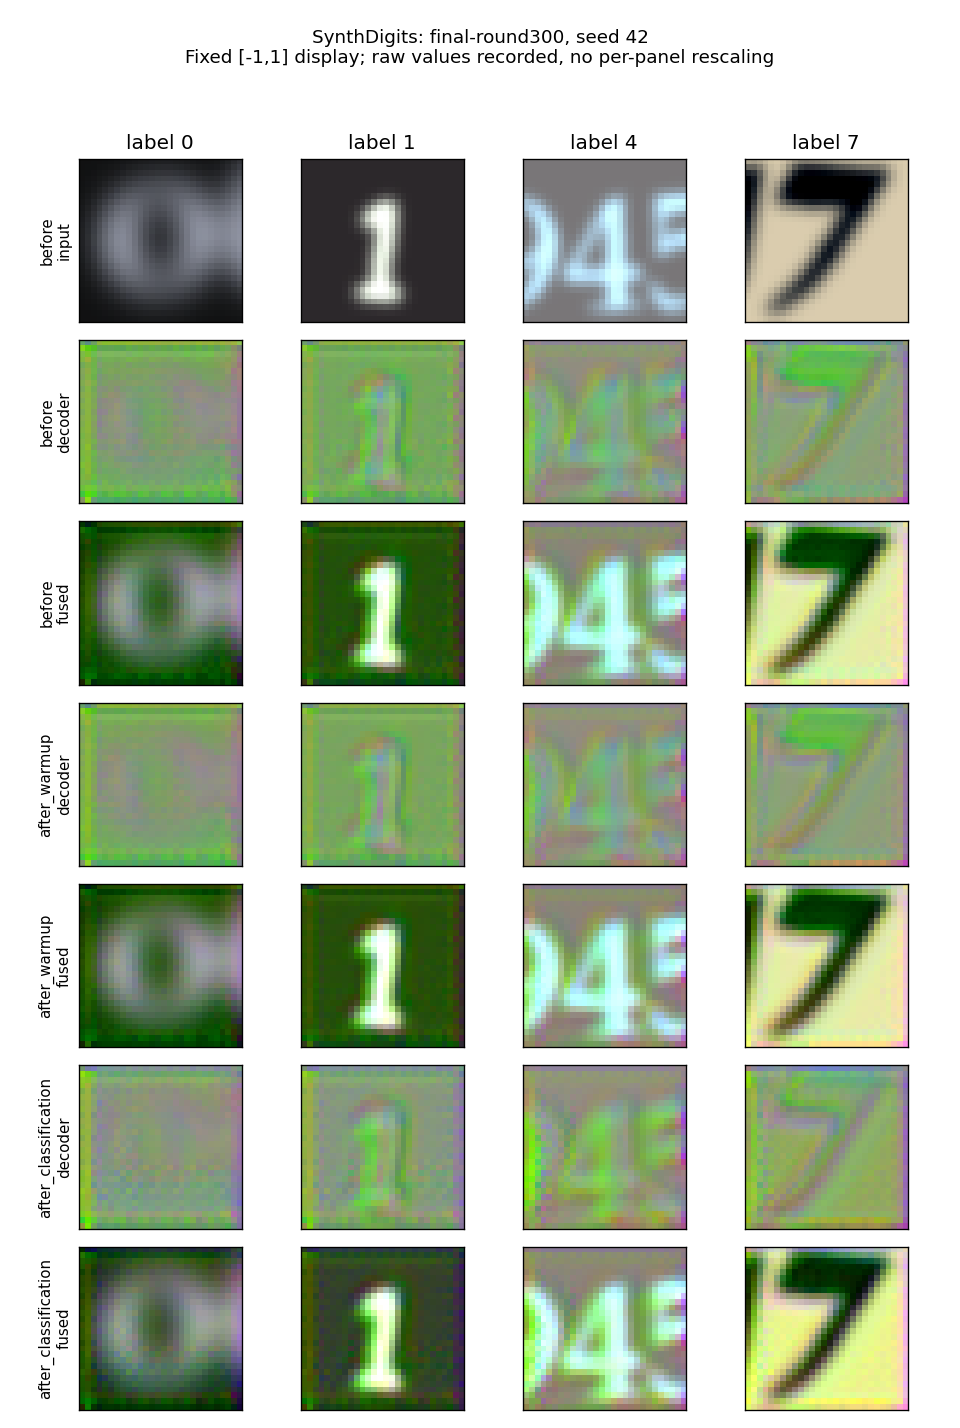
\includegraphics[width=.56in,trim=47.4bp 227.4bp 430.2bp 531.0bp,clip]{figures/digits/final-round300-SynthDigits.png} & 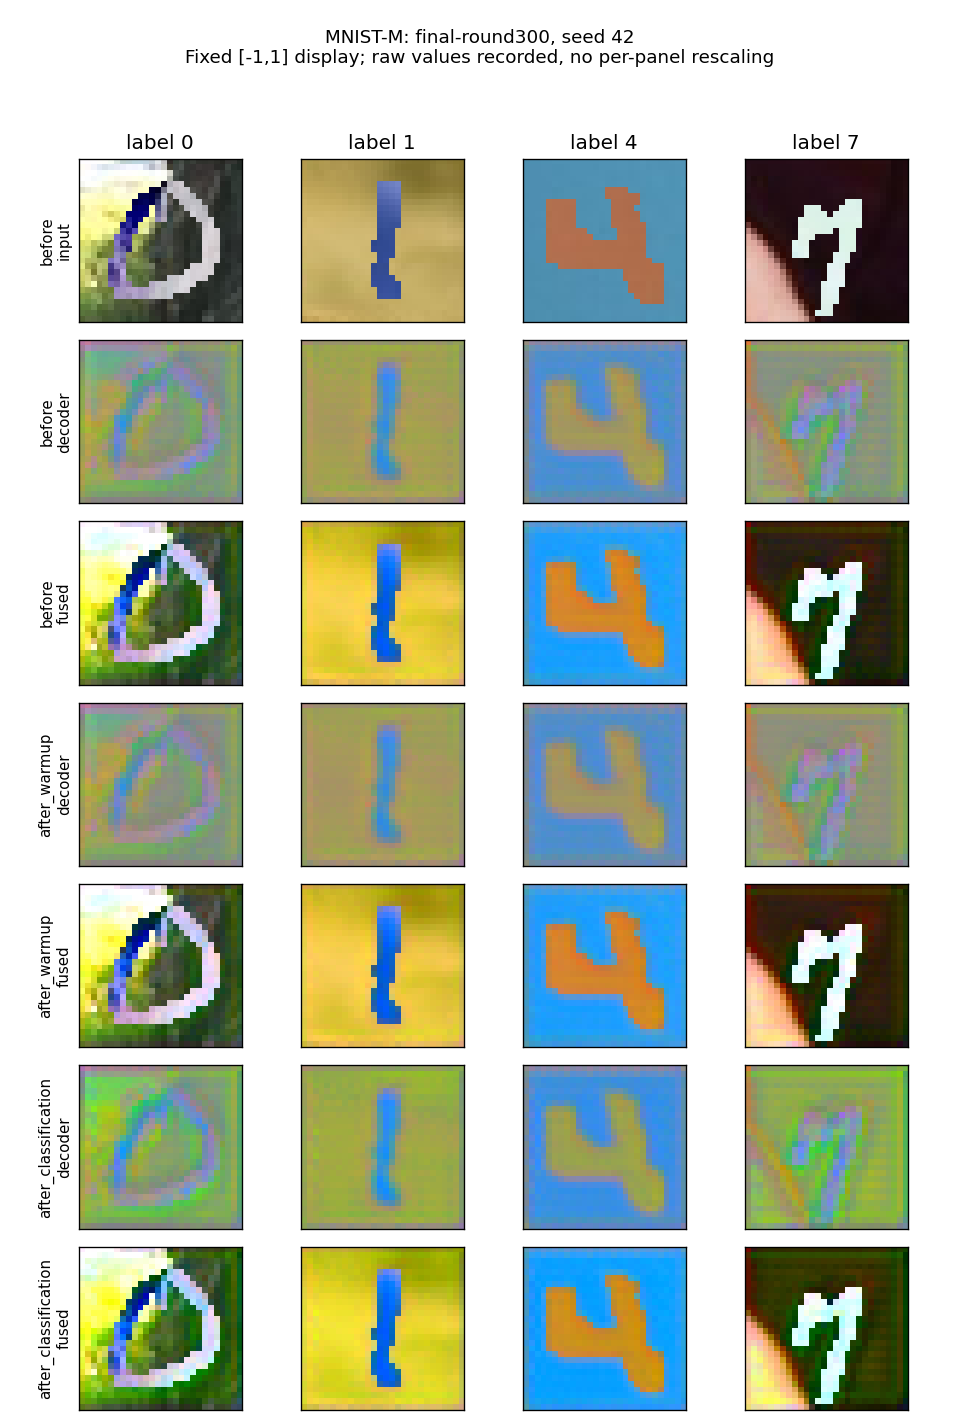
\includegraphics[width=.56in,trim=47.4bp 227.4bp 430.2bp 531.0bp,clip]{figures/digits/final-round300-MNIST-M.png} \\[-2pt]
\raisebox{.20in}{\scriptsize\shortstack[r]{After classification\\decoder}} & 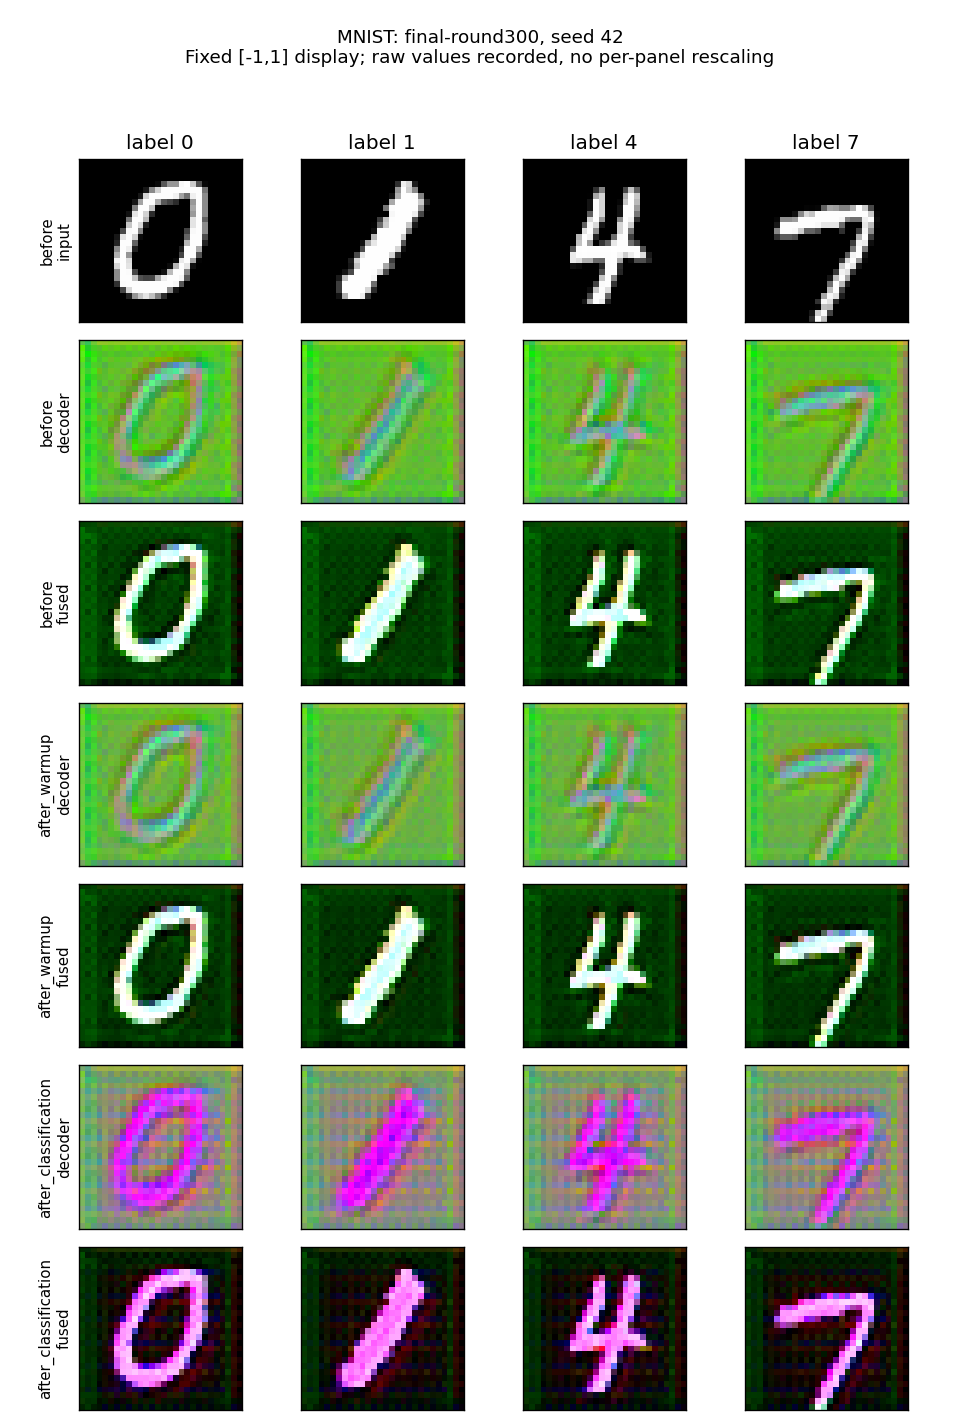
\includegraphics[width=.56in,trim=47.4bp 118.8bp 430.2bp 639.6bp,clip]{figures/digits/final-round300-MNIST.png} & 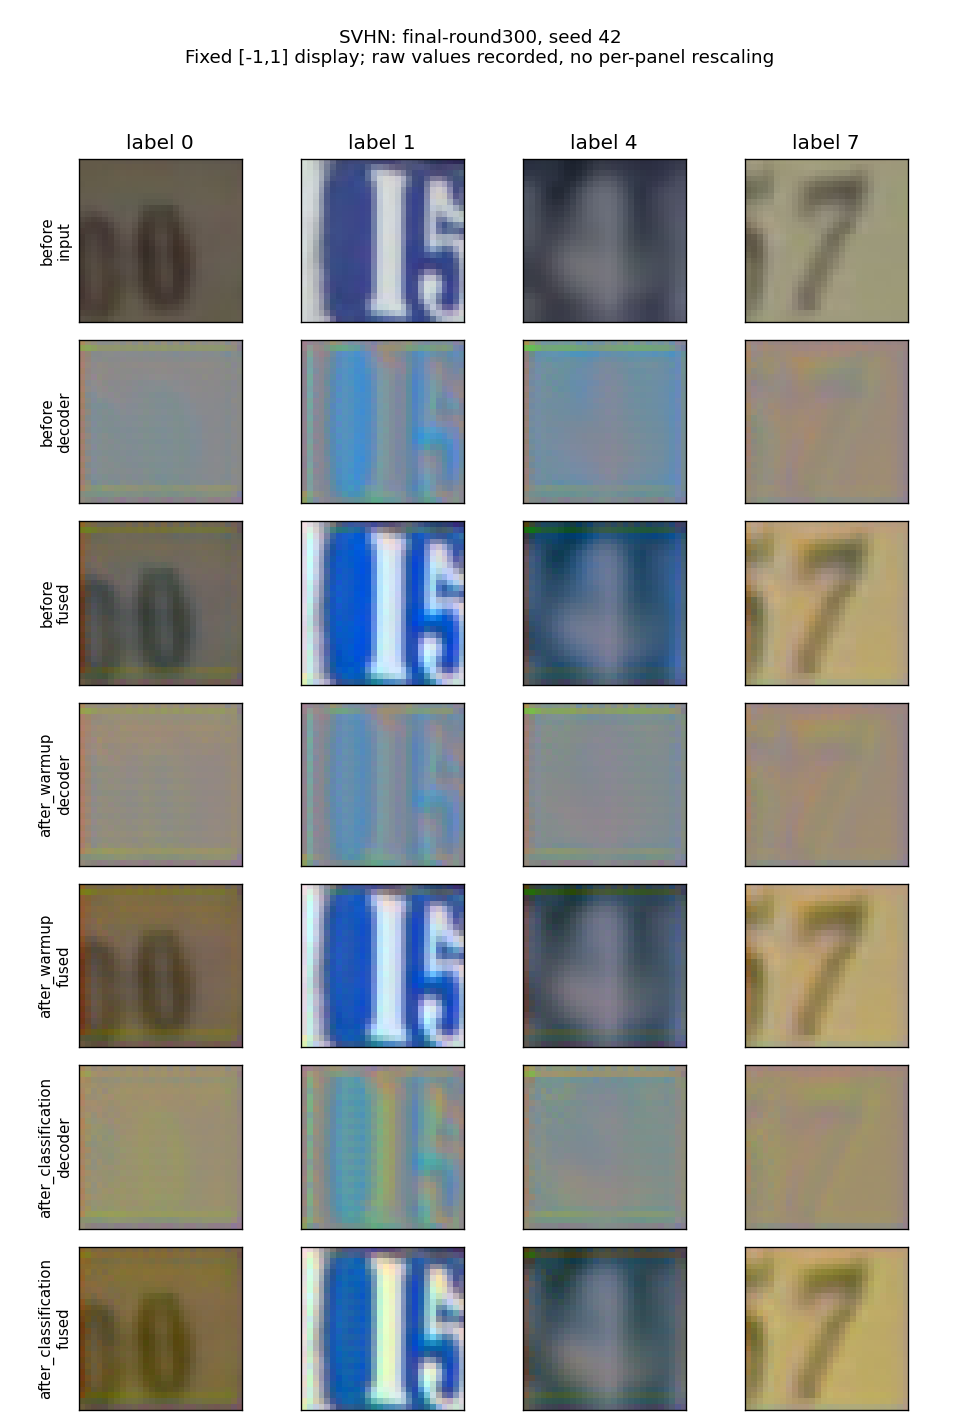
\includegraphics[width=.56in,trim=47.4bp 118.8bp 430.2bp 639.6bp,clip]{figures/digits/final-round300-SVHN.png} & 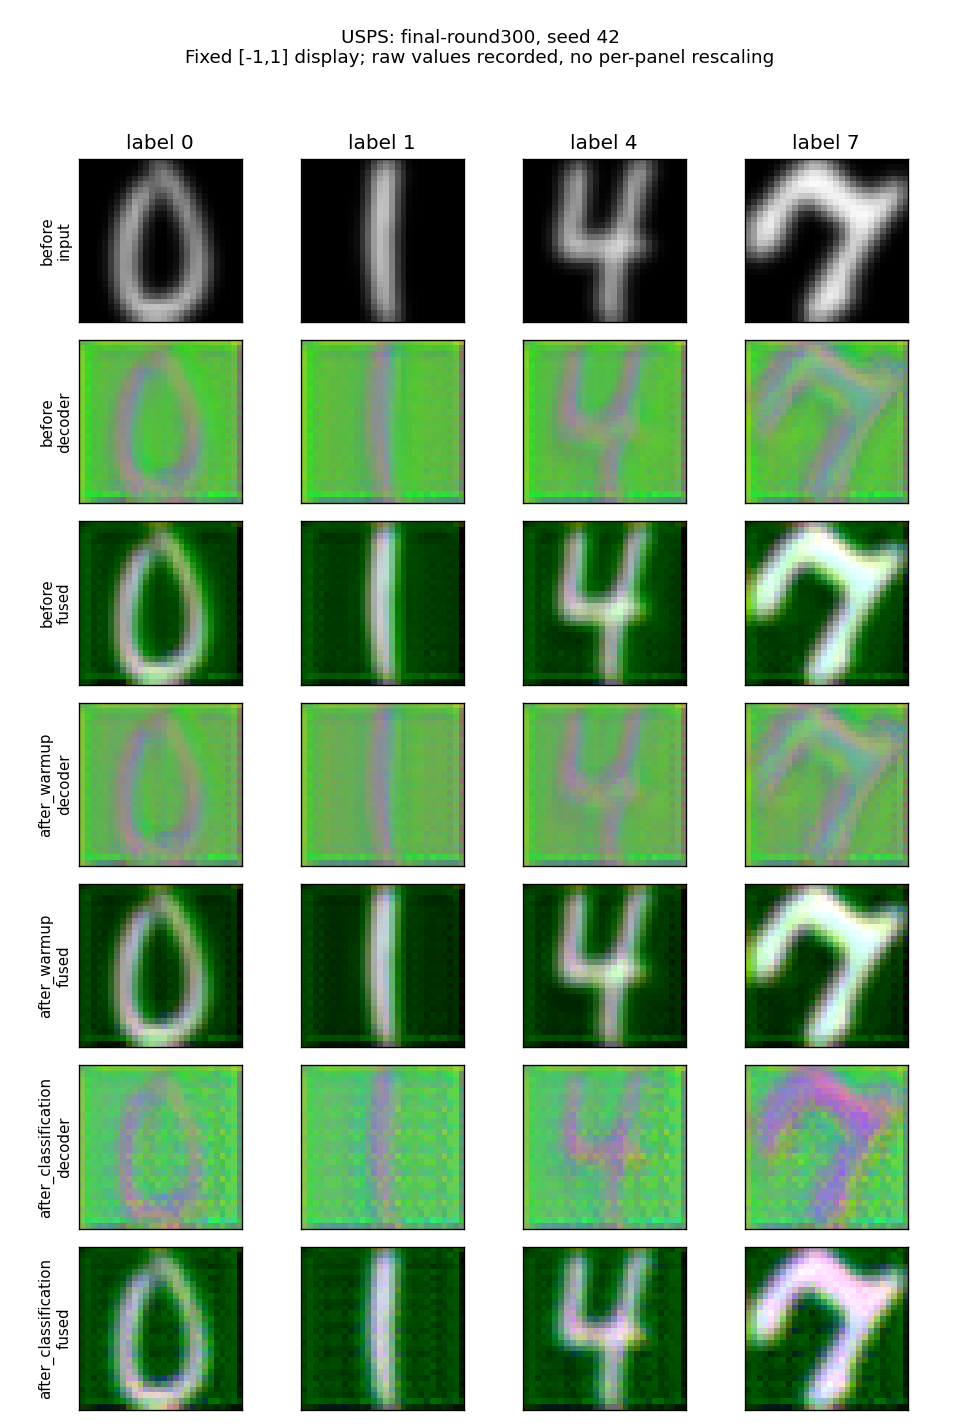
\includegraphics[width=.56in,trim=47.4bp 118.8bp 430.2bp 639.6bp,clip]{figures/digits/final-round300-USPS.png} & 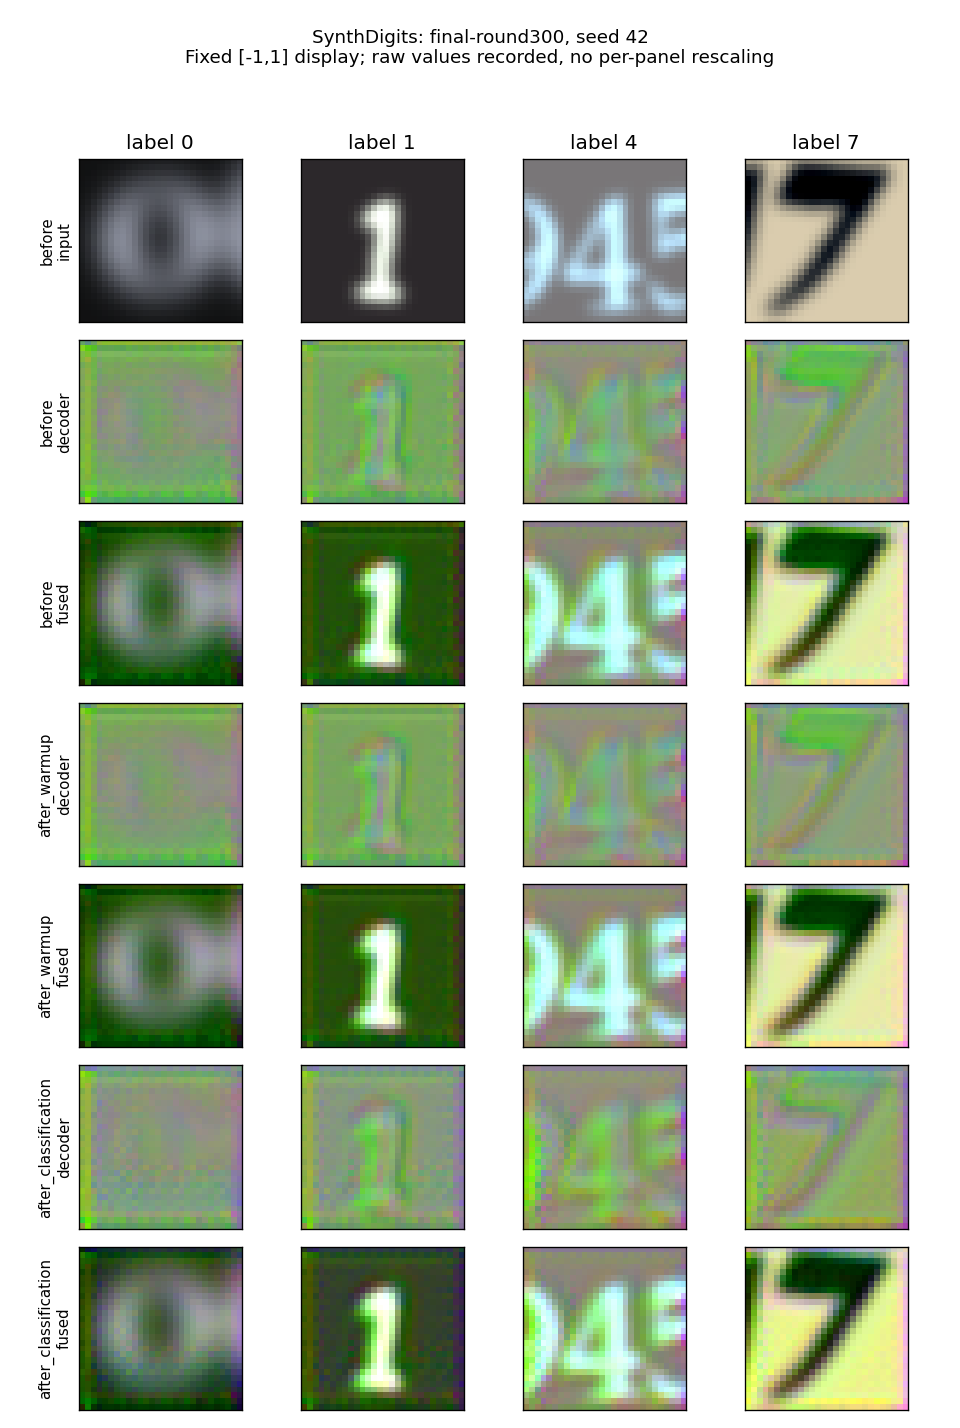
\includegraphics[width=.56in,trim=47.4bp 118.8bp 430.2bp 639.6bp,clip]{figures/digits/final-round300-SynthDigits.png} & 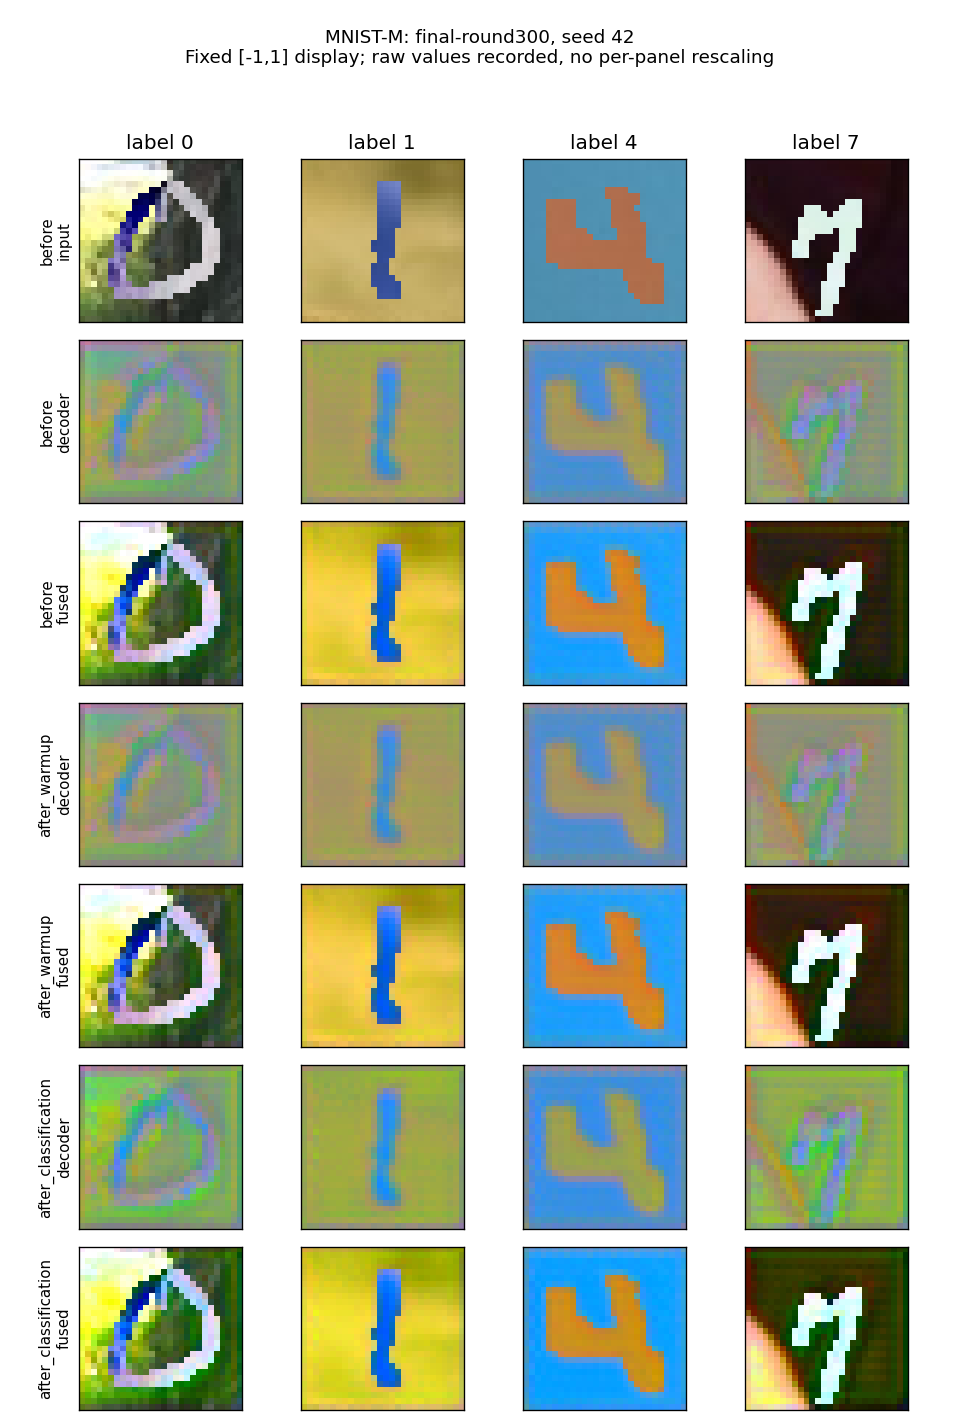
\includegraphics[width=.56in,trim=47.4bp 118.8bp 430.2bp 639.6bp,clip]{figures/digits/final-round300-MNIST-M.png} \\[-2pt]
\raisebox{.20in}{\scriptsize\shortstack[r]{After classification\\fused}} & 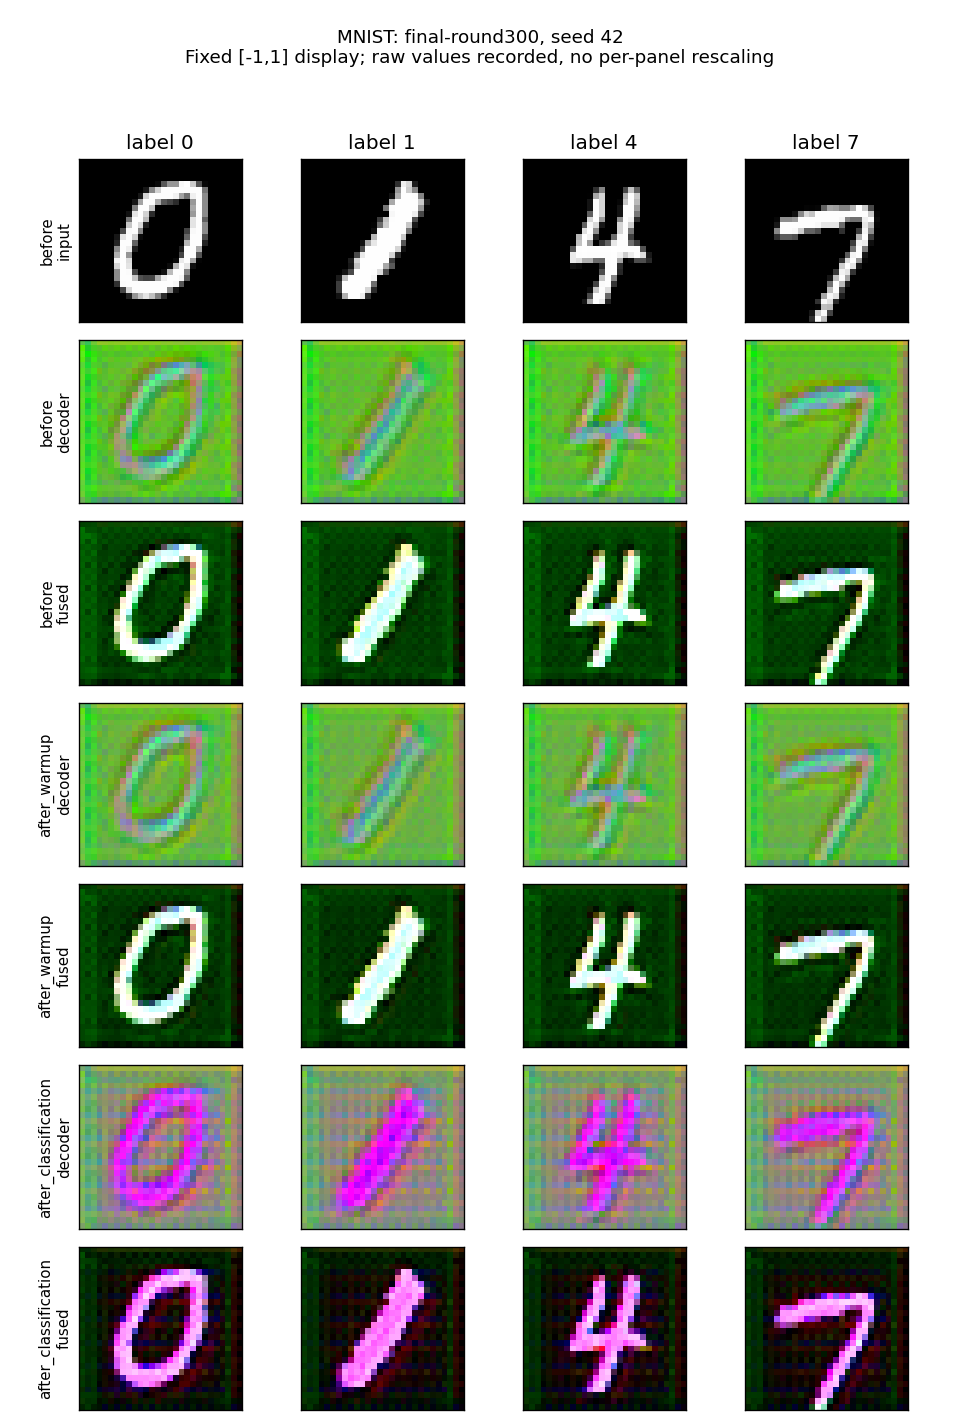
\includegraphics[width=.56in,trim=47.4bp 9.6bp 430.2bp 748.8bp,clip]{figures/digits/final-round300-MNIST.png} & 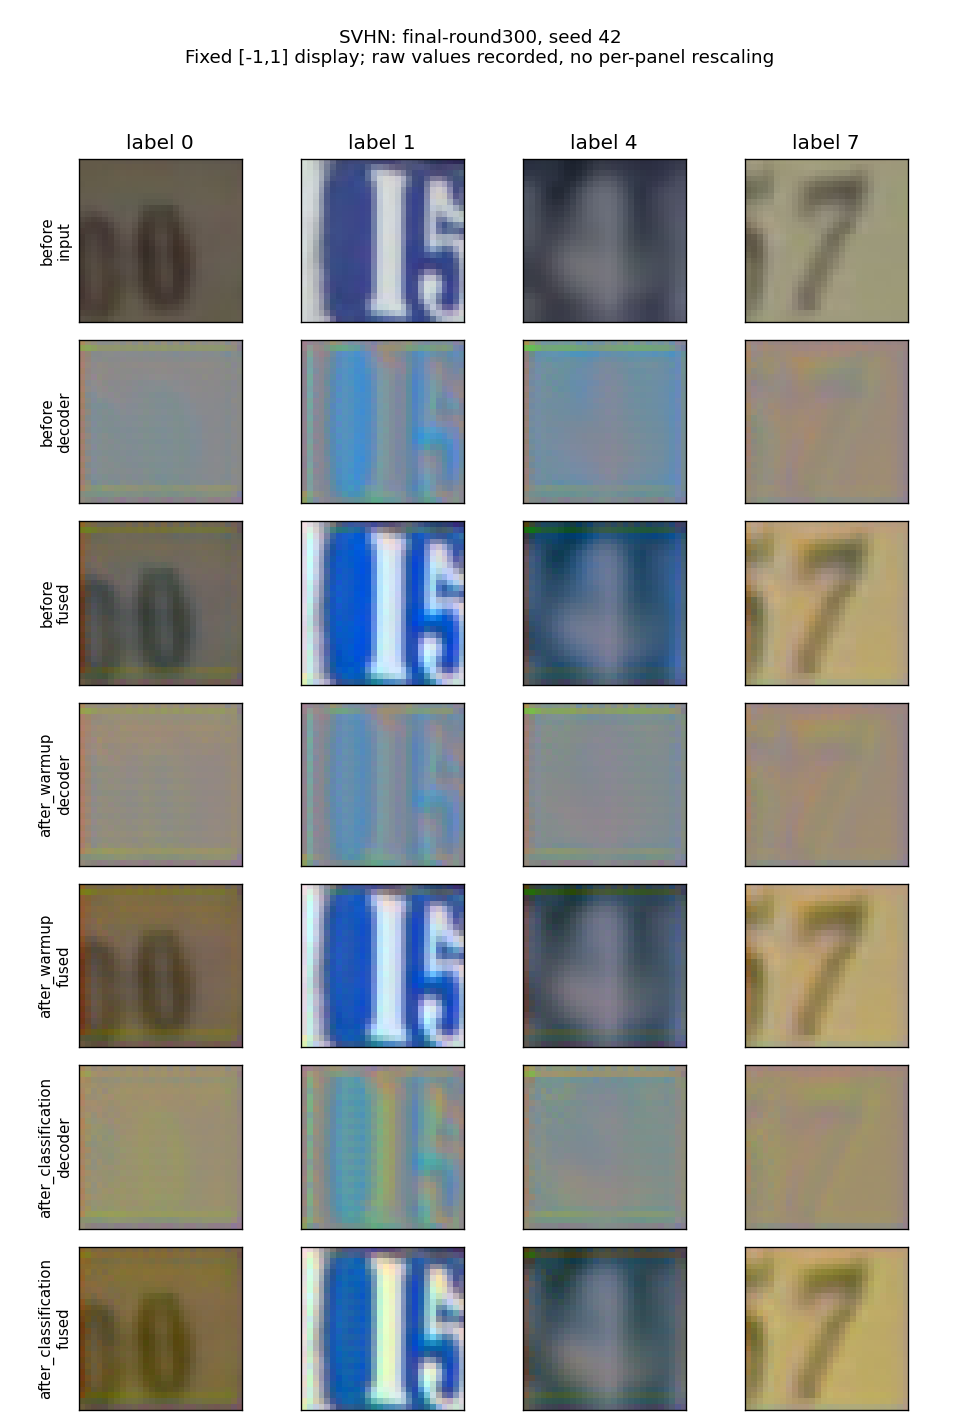
\includegraphics[width=.56in,trim=47.4bp 9.6bp 430.2bp 748.8bp,clip]{figures/digits/final-round300-SVHN.png} & 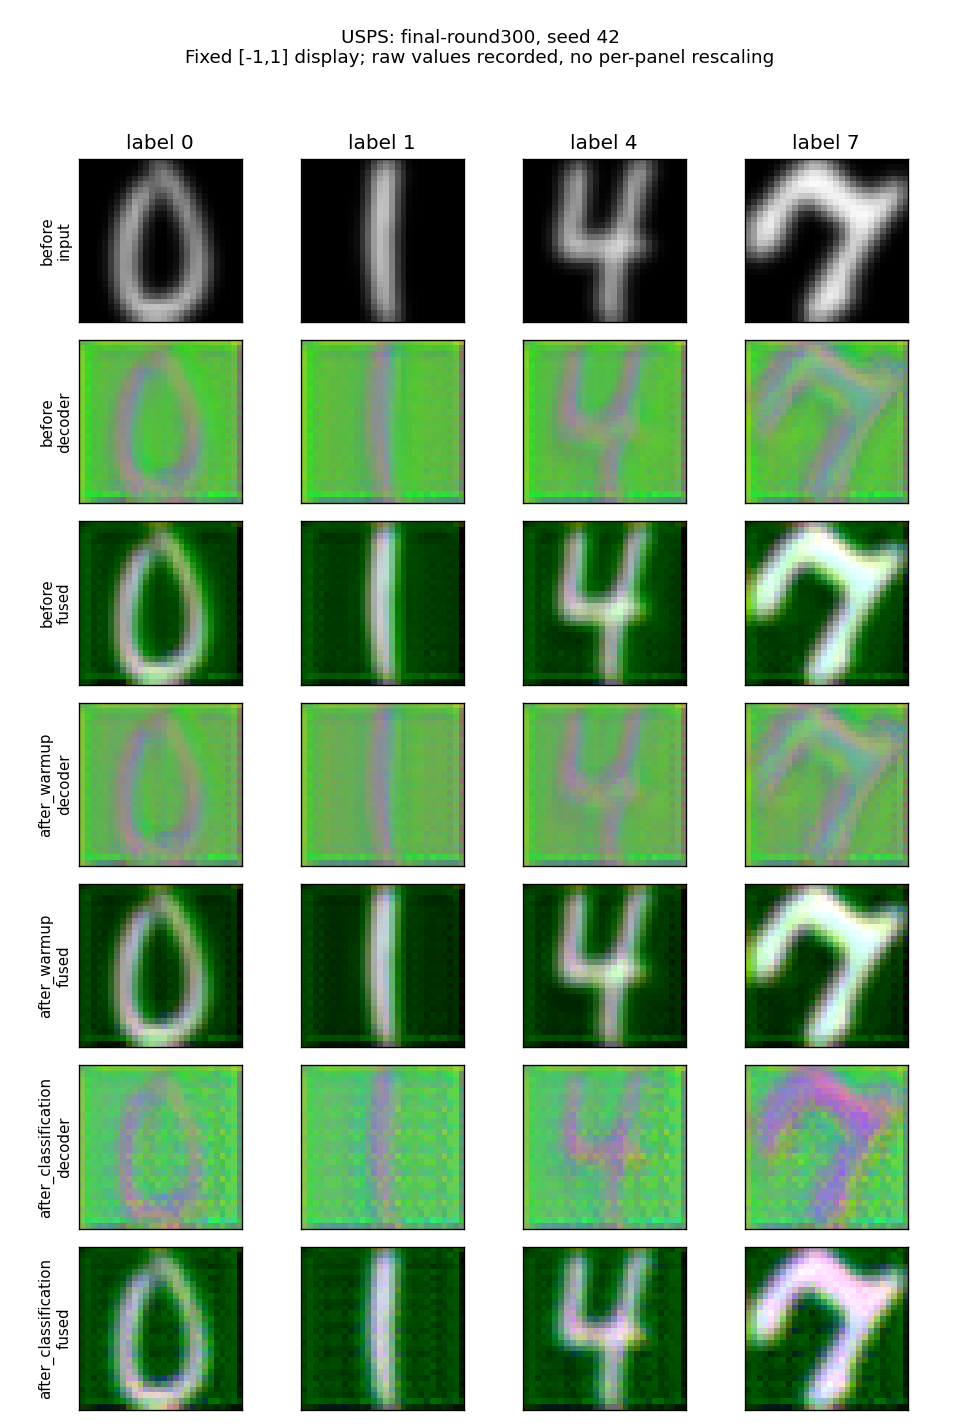
\includegraphics[width=.56in,trim=47.4bp 9.6bp 430.2bp 748.8bp,clip]{figures/digits/final-round300-USPS.png} & 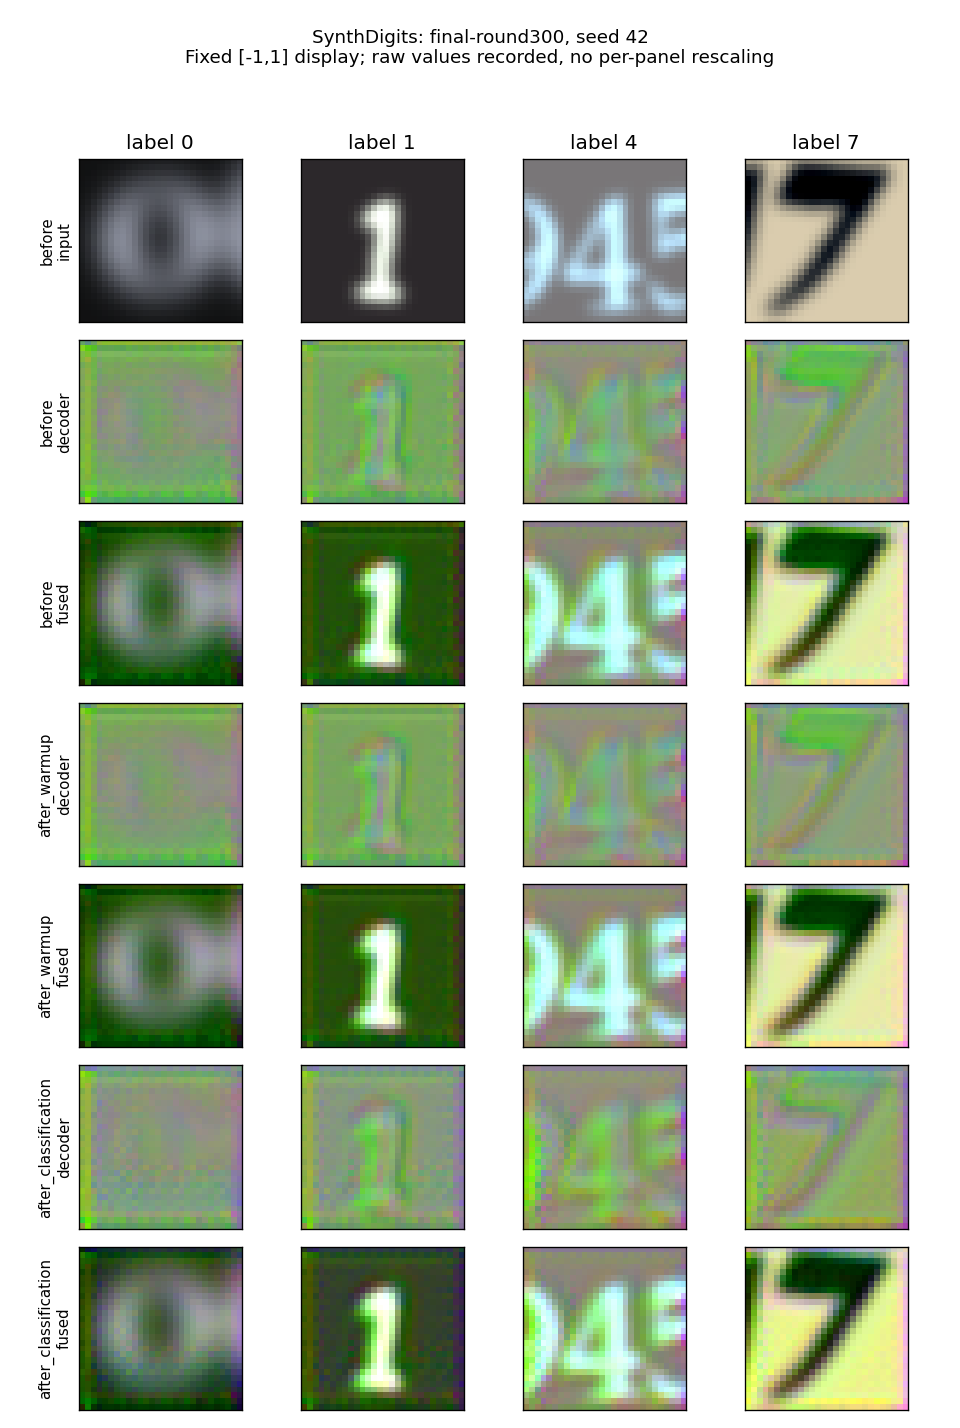
\includegraphics[width=.56in,trim=47.4bp 9.6bp 430.2bp 748.8bp,clip]{figures/digits/final-round300-SynthDigits.png} & 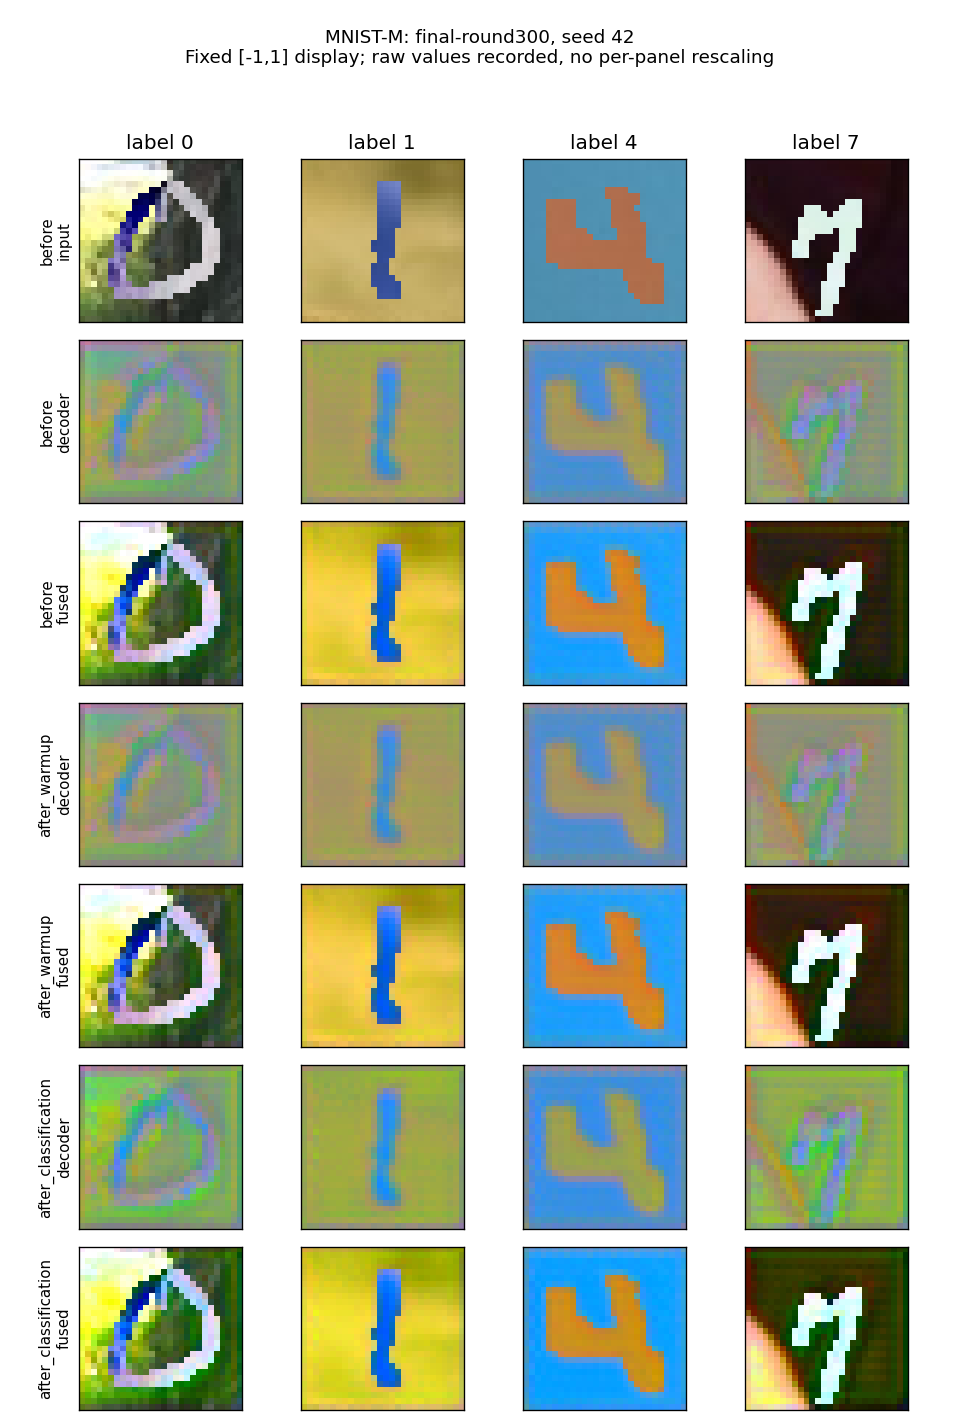
\includegraphics[width=.56in,trim=47.4bp 9.6bp 430.2bp 748.8bp,clip]{figures/digits/final-round300-MNIST-M.png} \\[-2pt]
\end{tabular}
\caption{Digits decoder probes from the final checkpoint, seed 42. Each column uses the first preselected class-0 example in that domain; the same example is shown throughout its local replay. Rows show the input and the decoder and fused outputs before adaptation, after warm-up, and after classification. All panels retain the fixed display range $[-1,1]$ of the archived grids; clipping is applied only for visualization, without panel-specific rescaling. Quantitative measurements use the raw, unclipped outputs.}
\label{fig:digits_decoder_probe}
\end{figure*}


\subsection{Component Ablations}
\label{app:digits_ablation}

How do the design choices affect the accuracy of the complete fusion
pipeline? We reuse the five full-model runs and train each of three variants
from scratch with the same five seeds, giving 15 additional runs of
300 rounds. The variants remove reconstruction warm-up, share the encoder,
or remove the original-input pathway. In the shared-encoder variant, all
clients start with the same encoder and uniformly average its state together
with the decoder and classifier after each round. The decoder-only variant
classifies $D(E_i(x))$ while retaining private encoders and warm-up.

All variants inherit the hyperparameters selected for the full pipeline,
without additional tuning: classifier SGD with learning rate 0.1,
encoder--decoder Adam with learning rate 0.0003, clipping at 10, batch size
32, and $d_z=64$. Training uses all 743 examples per domain and one
classification epoch per round; the full, shared-encoder, and decoder-only
variants additionally perform one warm-up epoch. Each final model is
evaluated once on the five domain test sets, containing 147,509 examples
in total. Uniform-domain accuracy is computed within each run.

\begin{table*}[t]
\coauthorcolor
\centering
\small
\setlength{\tabcolsep}{15pt}
\caption{Digits component ablations. Uniform-domain test accuracy at round 300 and paired differences are mean $\pm$ sample standard deviation over seeds 42--46. Positive differences favor the full pipeline. Bold marks the highest mean accuracy among the evaluated variants.}
\label{tab:digits_ablation}
\begin{tabular}{lcc}
\toprule
Variant & Uniform-domain accuracy (\%) & Full $-$ variant (pp) \\
\midrule
Full FusedSpaceFed & $85.86\pm0.85$ & -- \\
Without warm-up & $85.71\pm0.79$ & $+0.15\pm0.53$ \\
Shared encoder & $\boldsymbol{86.18\pm0.47}$ & $-0.32\pm0.58$ \\
Decoder output only & $84.86\pm0.58$ & $+1.00\pm1.22$ \\
\bottomrule
\end{tabular}
\end{table*}


Results are reported as mean $\pm$ sample standard deviation across five
paired seeds; differences are computed within each seed.
Removing warm-up also reduces the optimization budget and changes the Adam
state and minibatch order at the start of classification. This intervention
therefore measures the overall effect of removing the warm-up phase.

The complete pipeline achieves $85.86\%$ mean uniform-domain accuracy,
compared with $84.86\%$ when the original-input pathway is removed.
This 1.00-point average advantage supports combining the learned decoder
output with the original image. The no-warm-up and shared-encoder variants
obtain $85.71\%$ and $86.18\%$, respectively, showing smaller mean changes
under these interventions in the feature-heterogeneous Digits setting.

\subsection{Fixed-State Gradient Dispersion}
\label{app:digits_gradients}

Can the learned fusion pathway realize the variance--covariance reduction
condition in Equation~\eqref{eq:exact_decomp}? We compare original and fused
inputs at the initial and final checkpoints using identical classifier,
decoder, and private-encoder parameters. We use the same fixed training
probes as in Appendix~\ref{app:digits_decoder}, with no optimizer steps or
adaptation. For each client, we average the gradients of five minibatch
losses before computing cross-client dispersion.

The primary measurement freezes BatchNorm running statistics. A second
measurement uses batch statistics and restores all buffers before and after
each input pathway. These batch-statistic measurements condition the loss
on the fixed minibatches. Gradients are computed in float32 and accumulated
in float64. Table~\ref{tab:digits_gradient_decomposition} reports the terms
of the decomposition, which satisfy the identity to numerical precision.

\begin{table*}[t]
\coauthorcolor
\centering
\small
\setlength{\tabcolsep}{4pt}
\caption{Fixed-state classifier-gradient decomposition on Digits. Terms $\Gamma^{\mathrm{orig}}$, $\Gamma^{\mathrm{fused}}$, $B$, and $\Phi$ are means across five seeds. The ratio is computed within each seed and reported as mean $\pm$ sample standard deviation. The last column counts seeds satisfying $B+\Phi<0$. Frozen and Batch denote the two BatchNorm modes.}
\label{tab:digits_gradient_decomposition}
\begin{tabular}{llrrrrcc}
\toprule
Stage & BN & $\Gamma^{\mathrm{orig}}$ & $\Gamma^{\mathrm{fused}}$ & $B$ & $\Phi$ & $\Gamma^{\mathrm{fused}}/\Gamma^{\mathrm{orig}}$ & Reduced \\
\midrule
Initial & Frozen & $2.001\times10^{-2}$ & $2.012\times10^{-2}$ & $1.054\times10^{-3}$ & $-9.383\times10^{-4}$ & $1.006\pm0.013$ & 2/5 \\
Initial & Batch & $78.6571$ & $78.5144$ & $10.5506$ & $-10.6934$ & $0.998\pm0.004$ & 3/5 \\
Final & Frozen & $13.8595$ & $10.6770$ & $1.2951$ & $-4.4775$ & $0.792\pm0.253$ & 4/5 \\
Final & Batch & $6.732\times10^{-2}$ & $1.580\times10^{-3}$ & $5.700\times10^{-2}$ & $-0.1227$ & $0.148\pm0.141$ & 5/5 \\
\bottomrule
\end{tabular}

\par\vspace{10pt}
\coauthorcolor
\centering
\small
\setlength{\tabcolsep}{13pt}
\caption{Normalized and directional Digits gradient diagnostics, averaged across five seeds. Normalized dispersion is $\Gamma/(K^{-1}\sum_i\|g_i\|_2^2)$; cosine similarity is averaged over distinct pairs of client gradients. Orig.\ and Fused use identical model parameters and fixed training probes.}
\label{tab:digits_gradient_normalized}
\begin{tabular}{llrrrr}
\toprule
& & \multicolumn{2}{c}{Normalized dispersion} & \multicolumn{2}{c}{Pairwise cosine} \\
\cmidrule(lr){3-4}\cmidrule(lr){5-6}
Stage & BN & Orig. & Fused & Orig. & Fused \\
\midrule
Initial & Frozen & 0.7989 & 0.7988 & -0.0048 & -0.0049 \\
Initial & Batch & 0.7364 & 0.7370 & 0.0775 & 0.0763 \\
Final & Frozen & 0.7942 & 0.7996 & 0.0906 & 0.0440 \\
Final & Batch & 0.7966 & 0.7890 & 0.0218 & 0.0235 \\
\bottomrule
\end{tabular}
\end{table*}


At the final checkpoints, the mean per-seed ratio
$\Gamma^{\mathrm{fused}}/\Gamma^{\mathrm{orig}}$ is $0.792\pm0.253$
with frozen BatchNorm statistics and $0.148\pm0.141$ with batch statistics.
The reduction condition holds in four of five seeds and all five seeds,
respectively. These trained fusion pathways therefore provide empirical
instances of the absolute-dispersion reduction identified by the analysis.

To distinguish absolute dispersion from gradient scale and direction, we
also measure
$\Gamma/(K^{-1}\sum_i\|g_i\|_2^2)$ and the mean pairwise cosine similarity
of client gradients (Table~\ref{tab:digits_gradient_normalized}).
With frozen statistics, final-state normalized dispersion changes from
0.7942 to 0.7996 and mean pairwise cosine similarity from 0.0906 to 0.0440.
With batch statistics, the corresponding values change from 0.7966 to
0.7890 and from 0.0218 to 0.0235.
These results characterize a reduction in absolute dispersion, with
substantial sensitivity to gradient scale and BatchNorm statistics.
Both input pathways are evaluated at the same FusedSpaceFed state, whose
classifier was trained on fused inputs. Thus, the original-input pathway
is a fixed-state counterfactual; the cross-method measurements in
Section~\ref{sec:experiments} instead use each method's own final state.
